\documentclass[
  bibliography=totoc,     % Literatur im Inhaltsverzeichnis
  captions=tableheading,  % Tabellenüberschriften
  titlepage=firstiscover, % Titelseite ist Deckblatt
]{scrartcl}

% Paket float verbessern
\usepackage{scrhack}

% Warnung, falls nochmal kompiliert werden muss
\usepackage[aux]{rerunfilecheck}

% unverzichtbare Mathe-Befehle
\usepackage{amsmath}
% viele Mathe-Symbole
\usepackage{amssymb}
% Erweiterungen für amsmath
\usepackage{mathtools}

% Fonteinstellungen
\usepackage{fontspec}
% Latin Modern Fonts werden automatisch geladen
% Alternativ zum Beispiel:
%\setromanfont{Libertinus Serif}
%\setsansfont{Libertinus Sans}
%\setmonofont{Libertinus Mono}

% Wenn man andere Schriftarten gesetzt hat,
% sollte man das Seiten-Layout neu berechnen lassen
\recalctypearea{}

% deutsche Spracheinstellungen
\usepackage[ngerman]{babel}


\usepackage[
  math-style=ISO,    % ┐
  bold-style=ISO,    % │
  sans-style=italic, % │ ISO-Standard folgen
  nabla=upright,     % │
  partial=upright,   % │
  mathrm=sym,        % ┘
  warnings-off={           % ┐
    mathtools-colon,       % │ unnötige Warnungen ausschalten
    mathtools-overbracket, % │
  },                       % ┘
]{unicode-math}

% traditionelle Fonts für Mathematik
\setmathfont{Latin Modern Math}
% Alternativ zum Beispiel:
%\setmathfont{Libertinus Math}

\setmathfont{XITS Math}[range={scr, bfscr}]
\setmathfont{XITS Math}[range={cal, bfcal}, StylisticSet=1]

% Zahlen und Einheiten
\usepackage[
  locale=DE,                   % deutsche Einstellungen
  separate-uncertainty=true,   % immer Unsicherheit mit \pm
  per-mode=symbol-or-fraction, % / in inline math, fraction in display math
]{siunitx}

% chemische Formeln
\usepackage[
  version=4,
  math-greek=default, % ┐ mit unicode-math zusammenarbeiten
  text-greek=default, % ┘
]{mhchem}

% richtige Anführungszeichen
\usepackage[autostyle]{csquotes}

% schöne Brüche im Text
\usepackage{xfrac}

% Standardplatzierung für Floats einstellen
\usepackage{float}
\floatplacement{figure}{htbp}
\floatplacement{table}{htbp}

% Floats innerhalb einer Section halten
\usepackage[
  section, % Floats innerhalb der Section halten
  below,   % unterhalb der Section aber auf der selben Seite ist ok
]{placeins}

% Seite drehen für breite Tabellen: landscape Umgebung
\usepackage{pdflscape}

% Captions schöner machen.
\usepackage[
  labelfont=bf,        % Tabelle x: Abbildung y: ist jetzt fett
  font=small,          % Schrift etwas kleiner als Dokument
  width=0.9\textwidth, % maximale Breite einer Caption schmaler
]{caption}
% subfigure, subtable, subref
\usepackage{subcaption}

% Grafiken können eingebunden werden
\usepackage{graphicx}

% schöne Tabellen
\usepackage{booktabs}

% Verbesserungen am Schriftbild
\usepackage{microtype}

% Literaturverzeichnis
\usepackage[
  backend=biber,
]{biblatex}
% Quellendatenbank
\addbibresource{lit.bib}
\addbibresource{programme.bib}

% Hyperlinks im Dokument
\usepackage[
  german,
  unicode,        % Unicode in PDF-Attributen erlauben
  pdfusetitle,    % Titel, Autoren und Datum als PDF-Attribute
  pdfcreator={},  % ┐ PDF-Attribute säubern
  pdfproducer={}, % ┘
]{hyperref}
% erweiterte Bookmarks im PDF
\usepackage{bookmark}

% Trennung von Wörtern mit Strichen
\usepackage[shortcuts]{extdash}

%selber hinzugefügt
\usepackage{tabularray}
\UseTblrLibrary{booktabs}

\author{%
  Amelie Hater\\%
  \href{mailto:amelie.hater@tu-dortmund.de}{amelie.hater@tu-dortmund.de}%
  \and%
  Ngoc Le\\%
  \href{mailto:ngoc.le@tu-dortmund.de}{ngoc.le@tu-dortmund.de}%
}
\publishers{TU Dortmund – Fakultät Physik}

\subject{V207}
\title{Das Kugelfall\,-\,Viskosimeter nach Höppler}
\date{%
  Durchführung: 14.11.2023
  \hspace{3em}
  Abgabe: 20.11.2023
}

\begin{document}

\maketitle
\thispagestyle{empty}
\tableofcontents
\newpage

\section{Beschreibung}
\label{sec:Beschreibung}
Der digitale Versuchsaufbau kann wie folgt beschrieben werden: \\
Eine Feder hängt senkrecht zum Tisch aufgehängt auf einer bestimmten Höhe. 
An dem einen Ende der Feder ist ein Faden angebracht, der über ein Rad umgeleitet, parallel zum Tisch ausgezogen werden kann.
Die Auszugslänge kann durch ein unterliegendes Lineal gemessen werden und führt zum Auszug der Feder um dieselbe Länge.
Die zum Auszug benötigte Kraft wird gemessen und auf einem Bildschirm angezeigt. 

\section{Durchführung}
%Im Versuch werden mehrere Brückenschaltungen nach Schaltplan aufgebaut und die Nullmethode angewendet. Sobald die Spannung minimiert wurde, werden 
%die Widerstände $R_2$, $R_3$ und $R_4$ notiert. Diese Methode wird nacheinander auf die Wheatstonesche Brückenschaltung (), die Kapazitätsmessbrücke (Schaltplan in Abbildung (\ref{})) und die Induktivitätsmessbrücke (Schaltplan 
%in Abbildung (\ref{})) angewandt. Dabei sind bei jeder dieser Messbrücken zwei verschiedene, unbekannte Bauteile durch die Nullmethode zu bestimmen. Für jedes
%zu bestimmende Bauteil wird die Nullmethode 3 Mal mit verschiedenen Widerständen $R_2$ (und verschiedenen $C_2$ bei der Kapazitätsmessbrücke bzw. $L_2$ bei der
%Induktivitätsmessbrücke)
%
%Schaltplan in Abbildung (\ref{pic:Wheatstonesche_Brückenschaltung}) aufgebaut und die 
\subsection{Wheatstonesche Brücke}
Zuerst wird die Wheatstonesche Brückenschaltung nach Schaltplan in Abbildung (\ref{pic:Wheatstonesche_Brueckenschaltung}) aufgebaut. $R_3$ ist dabei ein Potentiometer
und $R_4$ ist durch $R_4 = 1000 \, \unit{\ohm} - R_3 $ festgelegt. Dann wird die Nullmethode angewendet.
Sobald die Spannung das Minimum erreicht, werden die Widerstände notiert. Diese Nullmethode wird insgesamt 3 Mal für einen unbekannten Widerstand angewendet, jeweils
mit unterschiedlichen $R_2$. Es werden zwei verschiedene unbekannte ohmsche Widerstände auf diese Weise bestimmt.  
\begin{figure}[H]
    \centering
    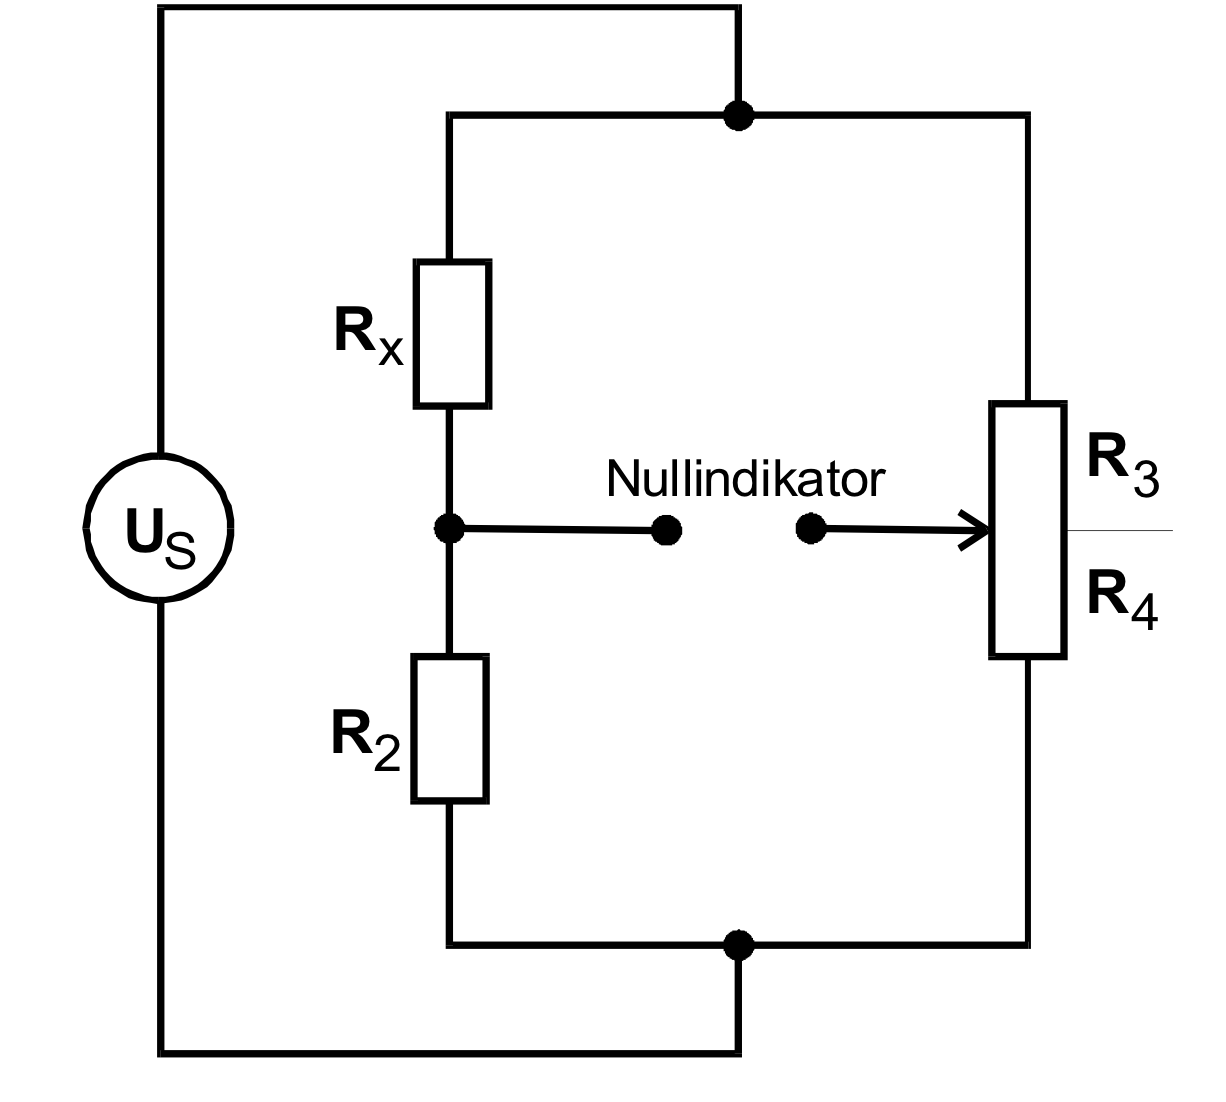
\includegraphics[width=0.4\linewidth]{Wheatstonesche.png}
    \caption{Schaltplan der Wheatstoneschen Brückenschaltung. Q\cite{anleitungV302}}
    \label{pic:Wheatstonesche_Brueckenschaltung}
\end{figure}
\subsection{Kapazitätsmessbrücke}
Die Kapazitätsmessbrücke wird nach Schaltplan in Abbildung (\ref{pic:Kapazitaetsmessbruecke}) aufgebaut und für $R_3$ bzw. $R_4$ wird dasselbe Potentiometer
verwendet wie bei der Wheatstoneschen Brücke. In diesem Teil des Versuches werden ebenfalls zwei unterschiedliche unbekannte Kapazitäten und zugehörige 
ohmsche Widerstände bestimmt durch je drei Messwerte. Bei jedem dieser Messwerte wird der Kondensator mit Kapazität $C_2$ und $R_2$ variiert, dann die Nullmethode durchgeführt und alle Kenngrößen
der bekannten Bauteile notiert. 
\begin{figure}[H]
    \centering
    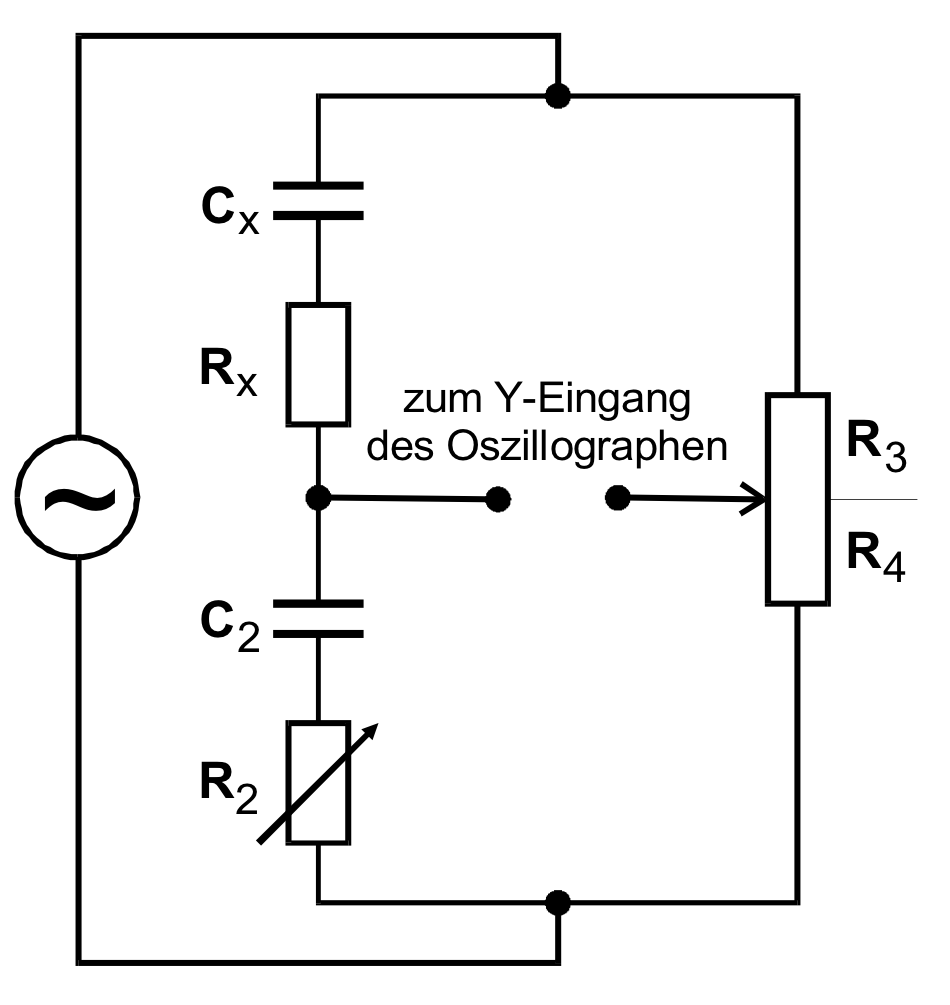
\includegraphics[width=0.4\linewidth]{Kapazitaet.png}
    \caption{Schaltplan der Kapazitätsmessbrücke. Q\cite{anleitungV302}}
    \label{pic:Kapazitaetsmessbruecke}
\end{figure}
\subsection{Induktivitätsmessbrücke}
Zur Messung zweier unbekannter Induktivitäten $L_x$ mit zugehörigem ohmschen Widerstand $R_x$ wird die Induktivitätsmessbrücke nach Schaltplan in Abbildung 
(\ref{pic:Induktivitaetsmessbruecke}) aufgebaut. Es werden die Kennzahlen zweier unterschiedlicher, unbekannter Spulen bestimmt, jeweils durch drei Messwerte bei 
denen $L_2$ und $R_2$ variiert wird. Zur Bestimmung von $R_3$ bzw. $R_4$ wird die Nullmethode angewandt und diese Widerstände notiert. 
\begin{figure}[H]
    \centering
    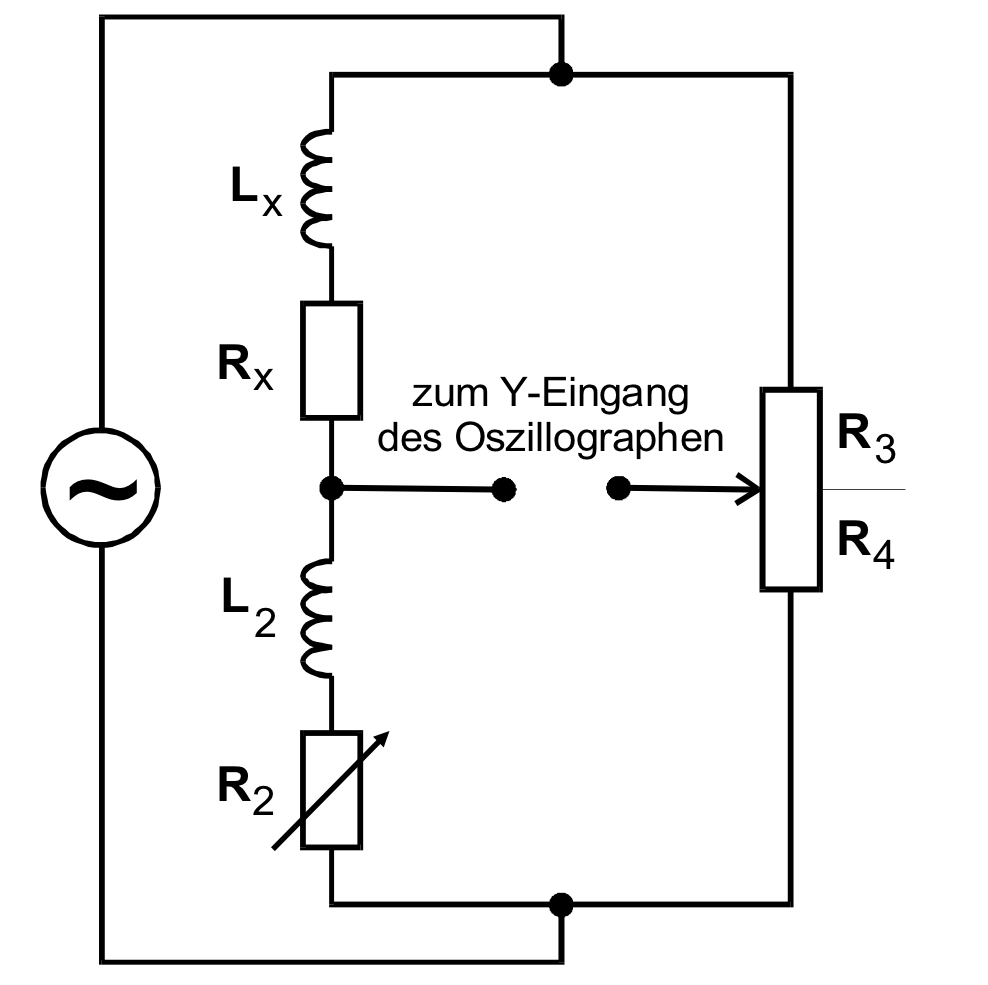
\includegraphics[width=0.4\linewidth]{Induktivitaet.png}
    \caption{Schaltplan der Induktivitätsmessbrücke. Q\cite{anleitungV302}}
    \label{pic:Induktivitaetsmessbruecke}
\end{figure} 
\subsection{Maxwell-Brücke}
Im folgenden Versuchsteil werden (idealerweise dieselben) zwei Induktivitäten $L_x$ mit zugehörigem ohmschen Widerstand $R_x$ erneut bestimmt mithilfe der 
Maxwell-Brücke. Der Schaltplan dieser Brücke ist in Abbildung (\ref{pic:Maxwell-Bruecke}) zu sehen. In diesem Versuchsteil sind $R_3$ und $R_4$ voneinander unabhängige
Potentiometer. Diese werden abwechselnd variiert bis das Spannungsminimum erreicht ist. Daraufhin werden alle Kennzahlen der Bauteile notiert. 
\begin{figure}[H]
    \centering
    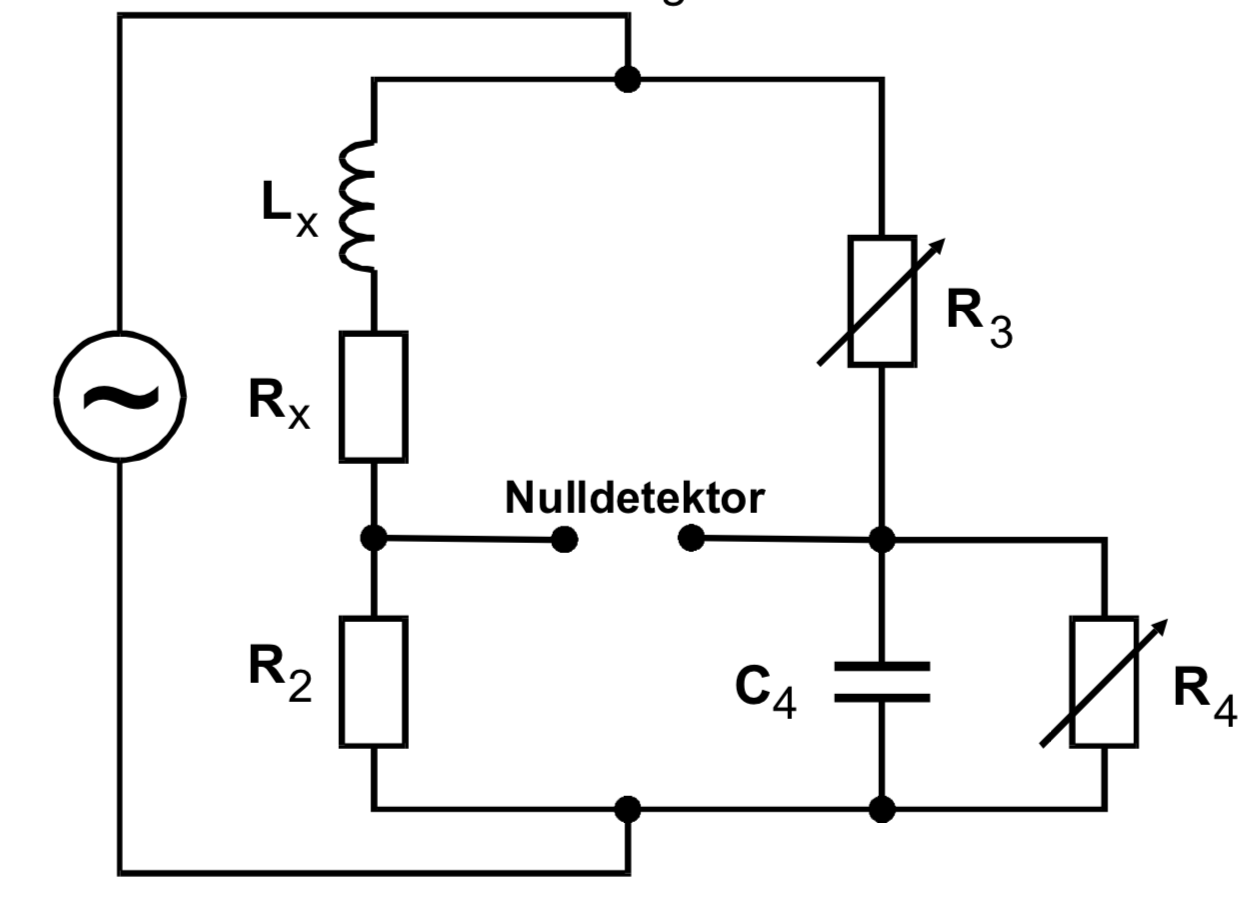
\includegraphics[width=0.4\linewidth]{Maxwell_Bruecke.png}
    \caption{Schaltplan der Maxwell-Brücke. Q\cite{anleitungV302}}
    \label{pic:Maxwell-Bruecke}
\end{figure} 
\subsection{Wien-Robinson-Brücke}
Die Wien-Robinson-Brücke wird gemäß Schaltplan in Abbildung (\ref{pic:WRB}) aufgebaut und für $R$ bzw. $R$' werden nur bekannte Widerstände verwendet. 
In diesem Teil des Versuchs wird die Frequenz der Quelle variiert und die resultierende Frequenz der Brückenspannung notiert. Im Bereich von 0 bis 500 Hz der Quellspannung 
werden die Messwerte in 50 Hz Schritten aufgenommen, von 500 bis 5000 Hz in 500 Hz Schritten. 
\begin{figure}[H]
    \centering
    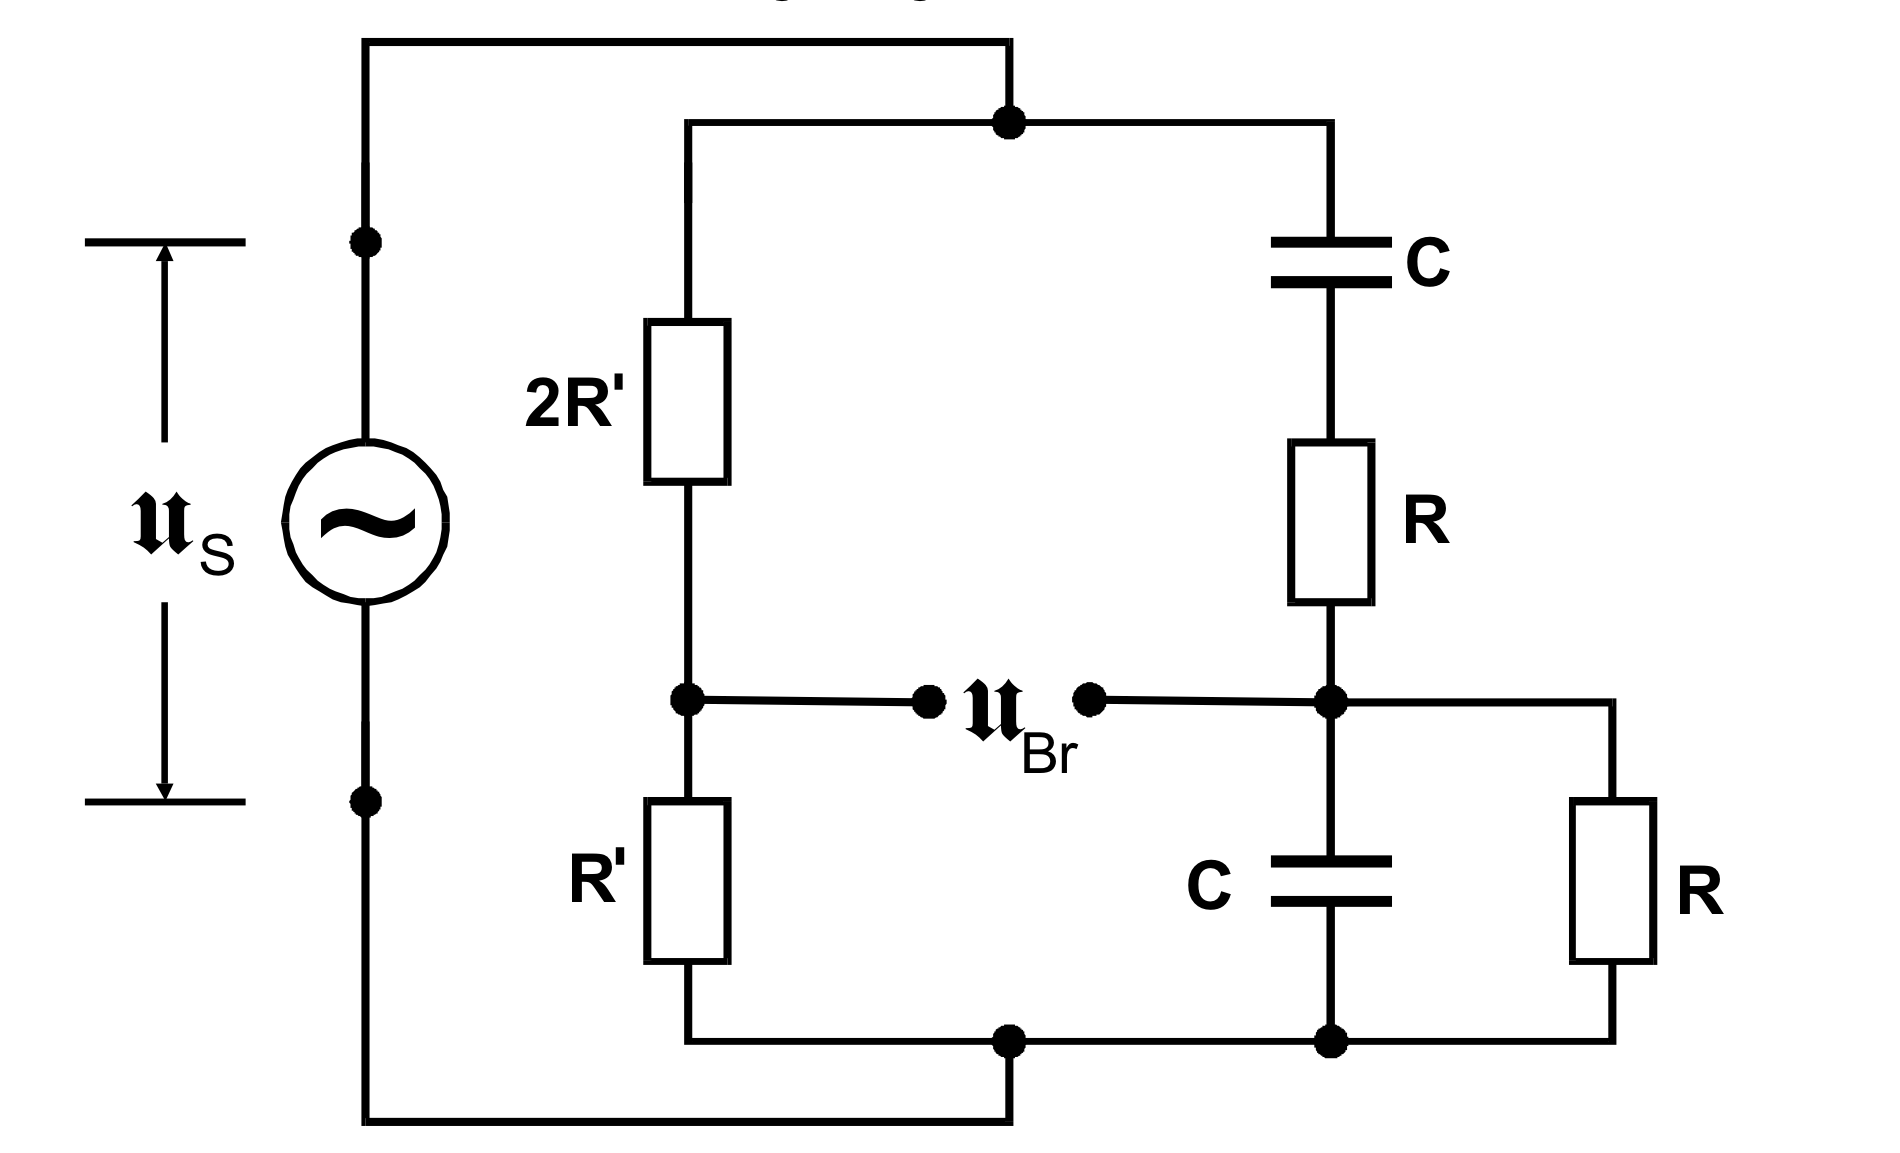
\includegraphics[width=0.4\linewidth]{Wienrobinson_Bruecke.png}
    \caption{Schaltplan der Wien-Robinson-Brücke. Q\cite{anleitungV302}}
    \label{pic:WRB}
\end{figure} 
%\subsection{Kirrfaktor}
%Der Klirrfaktor wird im Anschluss an den experimentellen Teil zur Qualitätseinschätzung des Oszilloskops bestimmt. 

% Brechungsindex theorie $n = 3,73$


\nocite{anleitungV407}
\section{Auswertung}
\label{sec:Auswertung}
Die zuerst gemessenen Werte des Nullstroms $I_0$ und des Dunkelstroms $I_{\text{D}}$ lauten
\begin{align*}
  I_0 &= 460\,\unit{\micro\ampere}\\
  I_{\text{D}} &= 2,8\,\unit{\nano\ampere}\,.
\end{align*}
Während der Messung des Dunkelstroms, ist das Photoelement so positioniert worden, dass es einer maximalen 
Störung der Lichtquellen ausgesetzt ist. Bei der Durchführung treffen im Allgemeinen nur kleinere Störungen auf
das Photoelement. Zusätzlich befindet sich die maximale Störung in einem kleinen Bereich, weswegen der Dunkelstrom im weiteren Verlauf der Auswertung vernachlässigt wird.
\\In der Tabelle \ref{tab:Messwerte} sind die gemessenen Photoströme in Abhängigkeit des Einfallswinkels $\alpha$ aufgelistet.
Um die Brechungsindizes für s- und p-polarisiteres Licht zu bestimmen, werden die Gleichungen (\ref{eqn:E_r_senkrecht}) und (\ref{eqn:E_r_parallel}) nach $n_{\text{s}}$ und $n_{\text{p}}$
umgestellt. Daraus ergeben sich
\begin{align}
  n_{\text{s}} &= \sqrt{\frac{E^2 - 2E\cos(2\alpha) + 1}{E^2- 2E + 1}} \label{eqn:n_s} \qquad {\text{und}}\\
  n_{\text{p}} &= \sqrt{\left(\frac{1+E}{1-E}\right)^2 \frac{1}{2\cos^2(\alpha)} + \sqrt{\frac{(1+E)^2}{4\cos^4(\alpha)(1-E)^4}- \frac{1}{(1-E)^2} \tan^2(\alpha)}} \label{eqn:n_p}\,.
  % n_{\text{p}} &= \sqrt{\frac{(1+E)^2}{(1-E)^2}\frac{1}{2\cos^2(\alpha)} + \frac{\sqrt{(1+E)^2-4\cos^2(\alpha)(1-E)^2\sin^2(\alpha)}}{2\cos^2(\alpha)(1-E)^2}}
\end{align}
Hierfür gilt $$E = \frac{E_{\text{ref}}}{E_{\text{ein}}} = \frac{I_{\text{ref}}(\alpha)}{I_0}\,.$$
\begin{table}[H]
  % \centering
  \caption{Gemessene Photoströme bei einem s- und p-polarisiertem Laser in Abhängigkeit vom Einfallswinkel $\alpha$.}
  \label{tab:Messwerte}
  \begin{tblr}{colspec={c c c|| c c c|| c c c}}
      \toprule
      $\alpha\,[°]$ & $I_{\text{ref, s}}\,[\unit{\micro\ampere}]$ & $I_{\text{ref, p}}\,[\unit{\micro\ampere}]$ & $\alpha\,[°]$ & $I_{\text{ref, s}}\,[\unit{\micro\ampere}]$ & $I_{\text{ref, p}}\,[\unit{\micro\ampere}]$ & $\alpha\,[°]$ & $I_{\text{ref, s}}\,[\unit{\micro\ampere}]$ & $I_{\text{ref, p}}\,[\unit{\micro\ampere}]$ \\
      \midrule  
      6   &   6   &   14  &   38  &   24  &   20  &   70  &   110 &   3   \\
      8   &   8   &   14  &   40  &   31  &   20  &   71  &   120 &   1   \\
      10  &   7   &   15  &   42  &   28  &   20  &   72  &   120 &   2,2 \\
      12  &   10  &   15  &   44  &   39  &   20  &   73  &   130 &   1,4 \\
      14  &   6   &   14  &   46  &   38  &   20  &   74  &   140 &   0,9 \\
      16  &   11  &   11  &   48  &   47  &   20  &   75  &   140 &   0,5 \\
      18  &   10  &   16  &   50  &   46  &   20  &   76  &   130 &   0,57\\
      20  &   10  &   16  &   52  &   55  &   19  &   77  &   150 &   0,76\\
      22  &   12  &   16  &   54  &   64  &   17  &   78  &   140 &   1,5 \\
      24  &   15  &   17  &   56  &   70  &   16  &   79  &   160 &   2,8 \\
      26  &   12  &   17  &   58  &   70  &   16  &   80  &   150 &   4,6 \\
      28  &   17  &   18  &   60  &   80  &   14  &   82  &   170 &   10  \\
      30  &   14  &   18  &   62  &   78  &   12  &   84  &   160 &   23  \\
      32  &   19  &   19  &   64  &   90  &   10  &   86  &   190 &   43  \\
      34  &   18  &   19  &   66  &   90  &   8   &   87  &   190 &   60  \\
      36  &   26  &   19  &   68  &   110 &   5   &   &   & \\      
      \bottomrule
  \end{tblr}
\end{table}
Die berechneten Brechungsindizes sind in der Tabelle \ref{tab:Brechungsindex} aufgeführt. Ohne die Berücksichtigung von systematischen Fehlern, ergibt sich für die gemittelten Brechungsindizes
\begin{align*}
  \overline{n_{\text{s}}} &= 2,1\pm 1,1\quad \text{und}\\
  \overline{n_{\text{p}}} &= 4\pm 6\,.
\end{align*}
Insbesondere bei dem p-polarisierten Filter handelt es sich um einen großen Fehlerbereich. Daher werden aufgrund der systematischen Fehler für das s-polarisierte Licht die Werte $n_{\text{s}} > 4$ und bei dem p-polarisiertem 
Licht alle Werte $n_{\text{p}} > 6$ vernachlässigt. Die daraus gemittelten Brechungsindizes sind
\begin{align*}
  \overline{n_{\text{s}}} &= 2,0\pm 0,9\quad \text{und}\\
  \overline{n_{\text{p}}} &= 2,4\pm 1,1\,.
\end{align*}
Die Messdaten sind in der Abbildung \ref{fig:plot} dargestellt. Hierbei ist $\sqrt{\sfrac{I(\alpha)}{I_0}}$ gegen $\alpha$ aufgetragen. Zusätzlich sind in der Abbildung
die Theoriekurven abgebildet, welche durch $\overline{n_{\text{s}}}$, $\overline{n_{\text{p}}}$ sowie den Gleichungen (\ref{eqn:E_r_senkrecht}) und (\ref{eqn:E_r_parallel}) bestimmt werden.
Außerdem wird anhand der Tabelle beim Minimum des p-polarisitem Lasers ein Brewsterwinkel von $\alpha_{\text{B}} = 75\,°$ abgelesen. Dieser ist ebenfalls in der Abbildung \ref{fig:plot} eingezeichnet.
Anhand dieses Brewsterwinkels lässt sich über die Gleichung (\ref{eqn:Brewster}) der theoretische Brechungsindex $$n = 3,73$$ ermitteln.
\begin{figure}[H]
  % \centering
  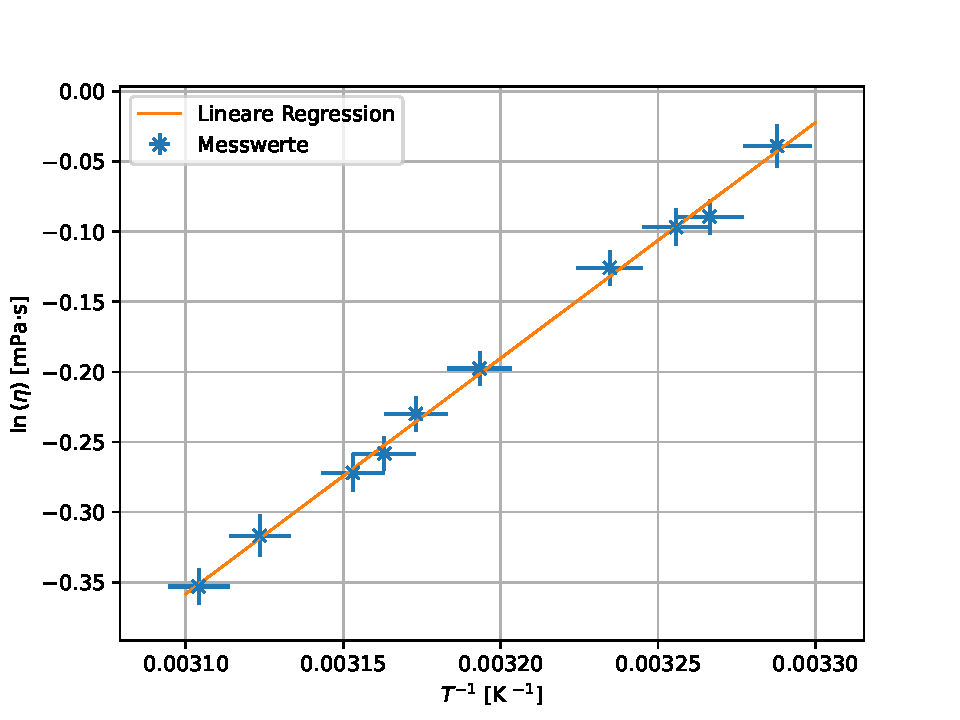
\includegraphics[width=\textwidth]{plot.pdf}
  \caption{Graphische Darstellung der Messwerte mit der Theoriekurve und markiertem Brewsterwinkel.}
  \label{fig:plot}
\end{figure}
\begin{table}[H]
    \centering
    \caption{Brechnete Brechungsindizes in Abhängigkeit des Winkels und der Intensität.}
    \label{tab:Brechungsindex}
    \begin{tblr}{colspec={c c c|| c c c|| c c c}}
        \toprule
        $\alpha\,[°]$ & $n_{\text{s}}$ & $n_{\text{p}}$ & $\alpha\,[°]$ & $n_{\text{s}}$ & $n_{\text{p}}$ & $\alpha\,[°]$ & $n_{\text{s}}$ & $n_{\text{p}}$ \\
        \midrule  
        6   &   1,00  &   1,37  & 38&   1,26  &   1,75  &   70  &   2,76 &   3,24\\
        8   &   1,01  &   1,38  & 40&   1,34  &   1,80  &   71  &   2,94 &   3,19\\
        10  &   1,01  &   1,40  & 42&   1,33  &   1,85  &   72  &   2,95 &   3,53\\
        12  &   1,02  &   1,40  & 44&   1,46  &   1,91  &   73  &   3,14 &   3,64\\
        14  &   1,02  &   1,39  & 46&   1,47  &   1,98  &   74  &   3,34 &   3,80\\
        16  &   1,03  &   1,35  & 48&   1,59  &   2,06  &   75  &   3,35 &   3,98\\
        18  &   1,04  &   1,44  & 50&   1,61  &   2,15  &   76  &   3,18 &   4,29\\
        20  &   1,05  &   1,45  & 52&   1,73  &   2,22  &   77  &   3,58 &   4,67\\
        22  &   1,06  &   1,47  & 54&   1,87  &   2,27  &   78  &   3,39 &   5,23\\
        24  &   1,09  &   1,50  & 56&   1,97  &   2,37  &   79  &   3,81 &   5,94\\
        26  &   1,08  &   1,52  & 58&   2,00  &   2,51  &   80  &   3,61 &   6,81\\
        28  &   1,12  &   1,56  & 60&   2,16  &   2,60  &   82  &   4,06 &   9,31\\
        30  &   1,12  &   1,58  & 62&   2,17  &   2,71  &   84  &   3,86 &   14,34\\
        32  &   1,17  &   1,63  & 64&   2,37  &   2,84  &   86  &   4,59 &   25,32\\
        34  &   1,18  &   1,66  & 66&   2,40  &   2,98  &   87  &   4,59 &   37,91\\
        36  &   1,25  &   1,69  & 68&   2,73  &   3,08  &   &   & \\      
        \bottomrule
    \end{tblr}
  \end{table}



\section{Diskussion}
\label{sec:Diskussion}
Die Messwerte weisen eine große Abweichung im Vergleich zu den Theoriewerten auf.  \\
Trotzdessen, dass $(4,46 \pm 0,18) \cdot 10^{-3} \,\,\unit{\kilo\gram\meter\squared}$ keinen Theoriewert hat, kann angenommen werden, dass 
dieser Wert ungenau ist, da der Stab 
als masselos angenommen wird. Dies verfälscht $I_{\text{Drill}}$ signifikant. Die Winkelrichtgröße 
$D = (21,0 \pm 0,8) \cdot 10^{-3} \,\,\unit{\newton\meter}$ kann auch als eine Größe mit großer Messunsicherheit angenommen
werden, da es nicht möglich war gleichzeitig den Auslenkungswinkel und die benötigte Kraft exakt zu bestimmen. Es könnte zu einem großen 
Fehler durch Messparalaxe gekommen sein, der je nach Betrachtungswinkel unterschiedlich groß wäre. Durch diesen Umstand sind auch sämtliche 
Größen, die von $D$ abgeleitet wurden, mit großen Fehlern behaftet. \\
Aufgrund der existierenden Reibung während des Versuchs, werden die 
Periodendauern kleiner als sie eigentlich ohne Reibung wären. Dies könnte erklären, warum die gemessenen Werte durchgehend kleiner sind als die 
Theoriewerte. Außerdem kommt durch die Reaktionszeit der messenden Person eine weitere Ungenauigkeit hinzu, die sämtliche gemessenen 
Trägheitsmomente betrifft.\\
Das Trägheitsmoment der Scheibe $(1,85 \pm 0,07) \cdot 10^{-3} \,\,\unit{\kilo\gram\meter\squared}$ hat eine Abweichung von $37,95 \,\,\%$ 
zum Theoriewert $(2,552 \pm 0,006) \cdot 10^{-3} \,\,\unit{\kilo\gram\meter\squared}$.\\
Das Trägheitsmoment der Kugel $(1,90 \pm 0,08) \cdot 10^{-3} \,\,\unit{\kilo\gram\meter\squared}$ hat eine prozentuale 
Abweichung von $32,84 \,\,\%$ zum Theoriewert $(2,524 \pm 0,007) \cdot 10^{-3} \,\,\unit{\kilo\gram\meter\squared}$. \\
Als zusätzliche Fehlerquelle kommt bei der Berechnung des Trägheitsmoments der Puppe hinzu, dass die Periodendauer so klein war, dass selbst eine
Messung von $5\,T$ ungenau war. Das Trägheitsmoment der Puppe in Position 1 beträgt $(0,2 \pm 0,008) \cdot 10^{-3}\,\, \unit{\kilo\gram\meter\squared}$.
 Die Abweichung ist $31,00 \,\,\%$ zum Theoriewert von $(0,262 \pm 0,025) \cdot 10^{-3}\,\, \unit{\kilo\gram\meter\squared}$.\\
Das Trägheitsmoment der Puppe in Position 2 ist $ (0,491 \pm 0,020) \cdot 10^{-3}\,\, \unit{\kilo\gram\meter\squared}$ und die Abweichung beträgt 46,64 \,\,\% zum Theoriewert 
von $(0,72 \pm 0,05) \cdot 10^{-3}\,\, \unit{\kilo\gram\meter\squared}$.\\
Das Verhältnis vom Trägheitsmoment der Puppe in Position 1 zu dem in Position 2 ist $\frac{I_{\text{Pos1}}}{I_{\text{Pos2}}} = 0,4073$. Das
Verhältnis der Theorieträgheitsmomente ist $\frac{I_{\text{Pos1,theo}}}{I_{\text{Pos2,theo}}} = 0,3639$. Die Abweichung des gemessenen Verhältnis im
Vergleich zum theoretischen Verhältnis beträgt $10,66 \,\,\%$. Diese Abweichung ist deutlich geringer als die Abweichung der einzelnen Trägheitsmomente 
zum Theoriewert. 
 
\section{Originaldaten}
\label{sec:Originaldaten}
% \begin{figure}[H]
%   \centering
%   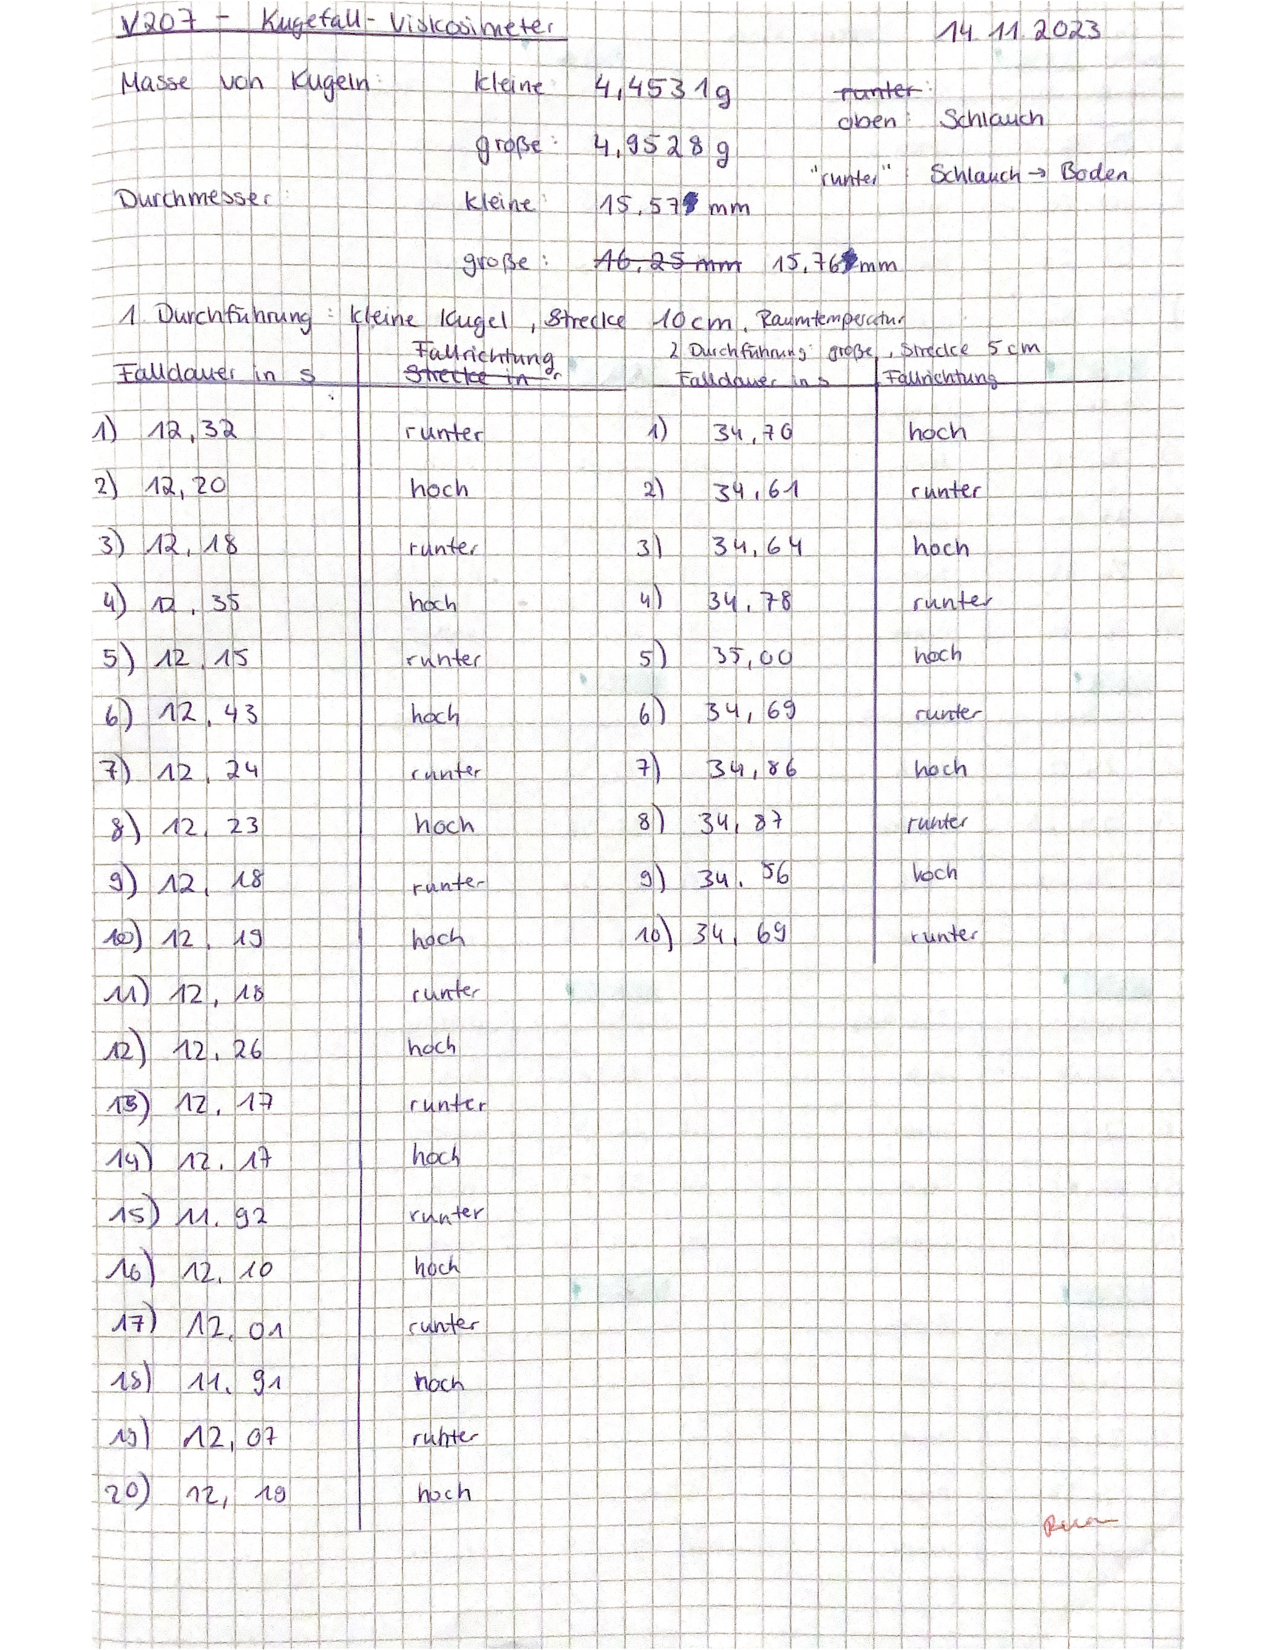
\includegraphics[width=\textwidth]{Messwerte_1.pdf}
%   \label{fig:Messungen}
% \end{figure}
% \begin{figure}[H]
    %   \centering
    %   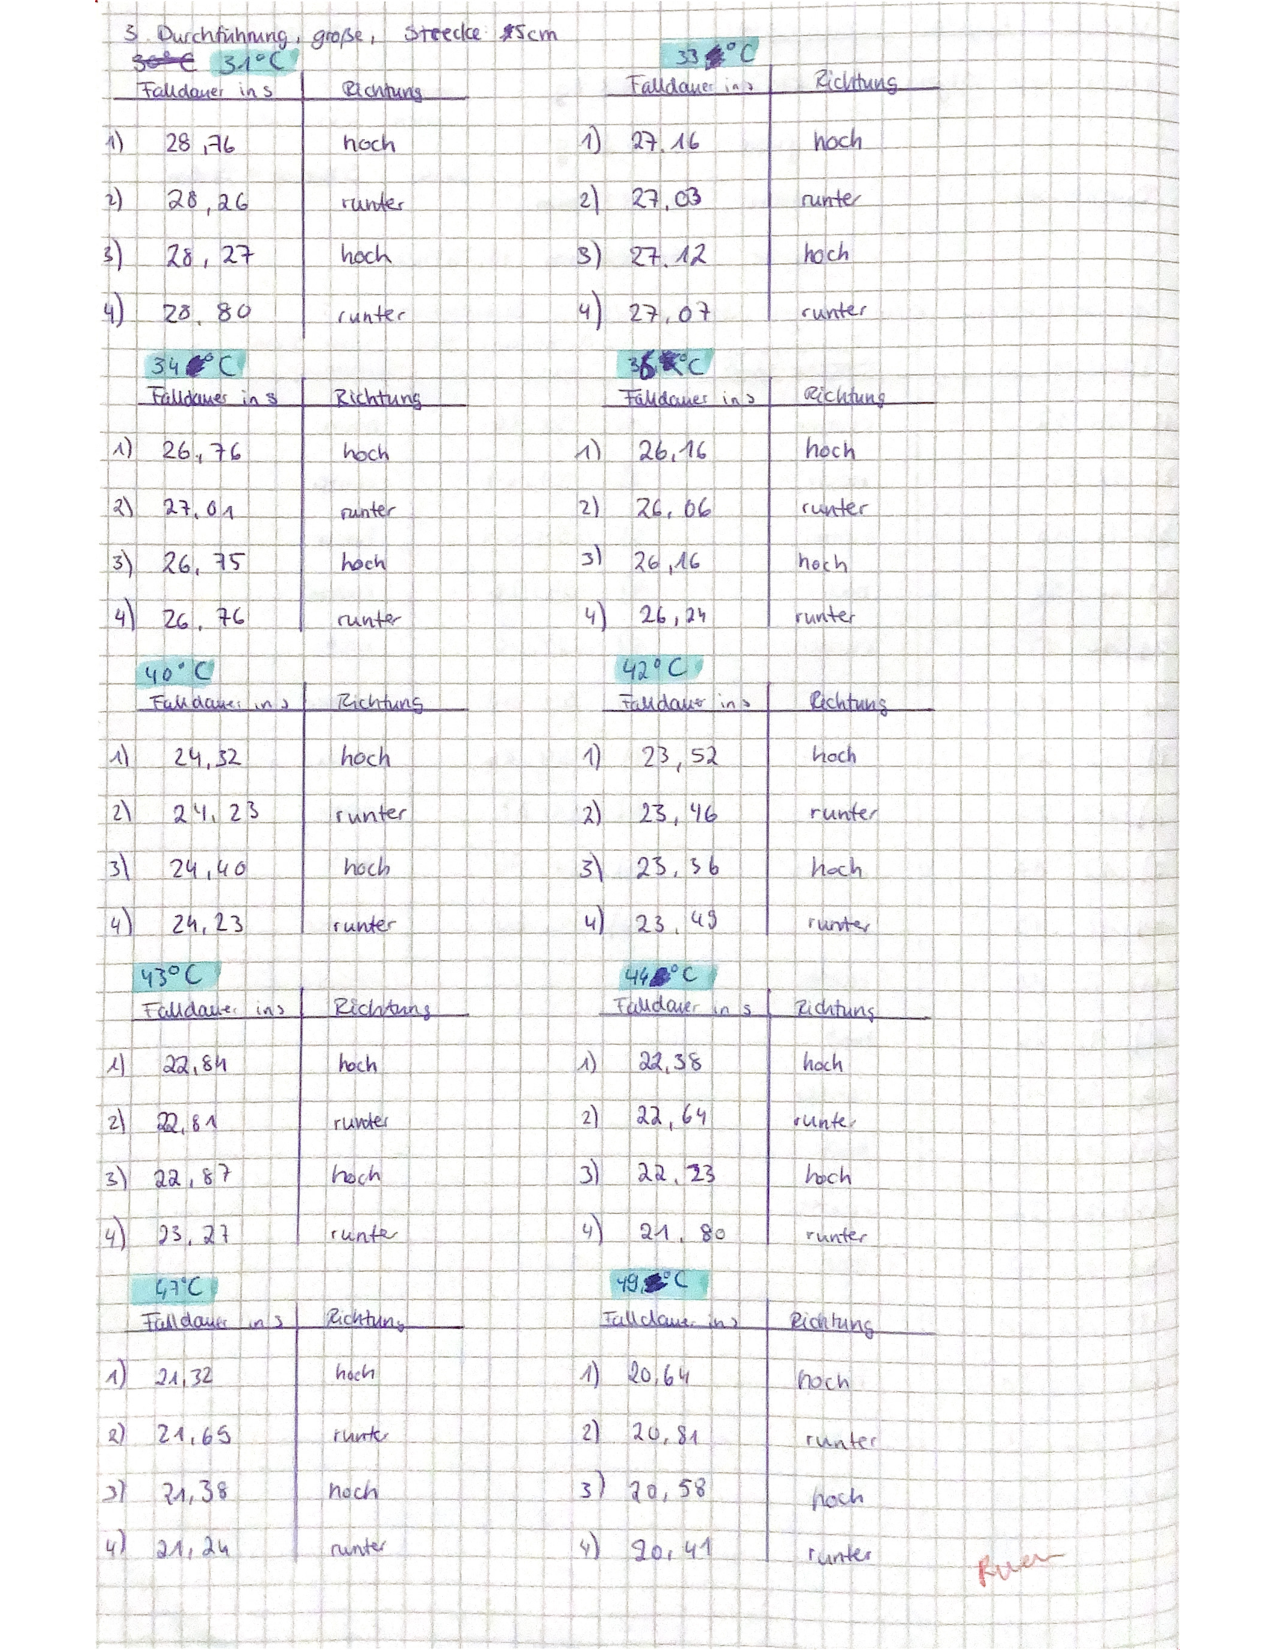
\includegraphics[width=\textwidth]{Messwerte_2.pdf}
    %   \label{fig:Messungen}
% \end{figure}
%\begin{figure}[H]
%   \centering
    %   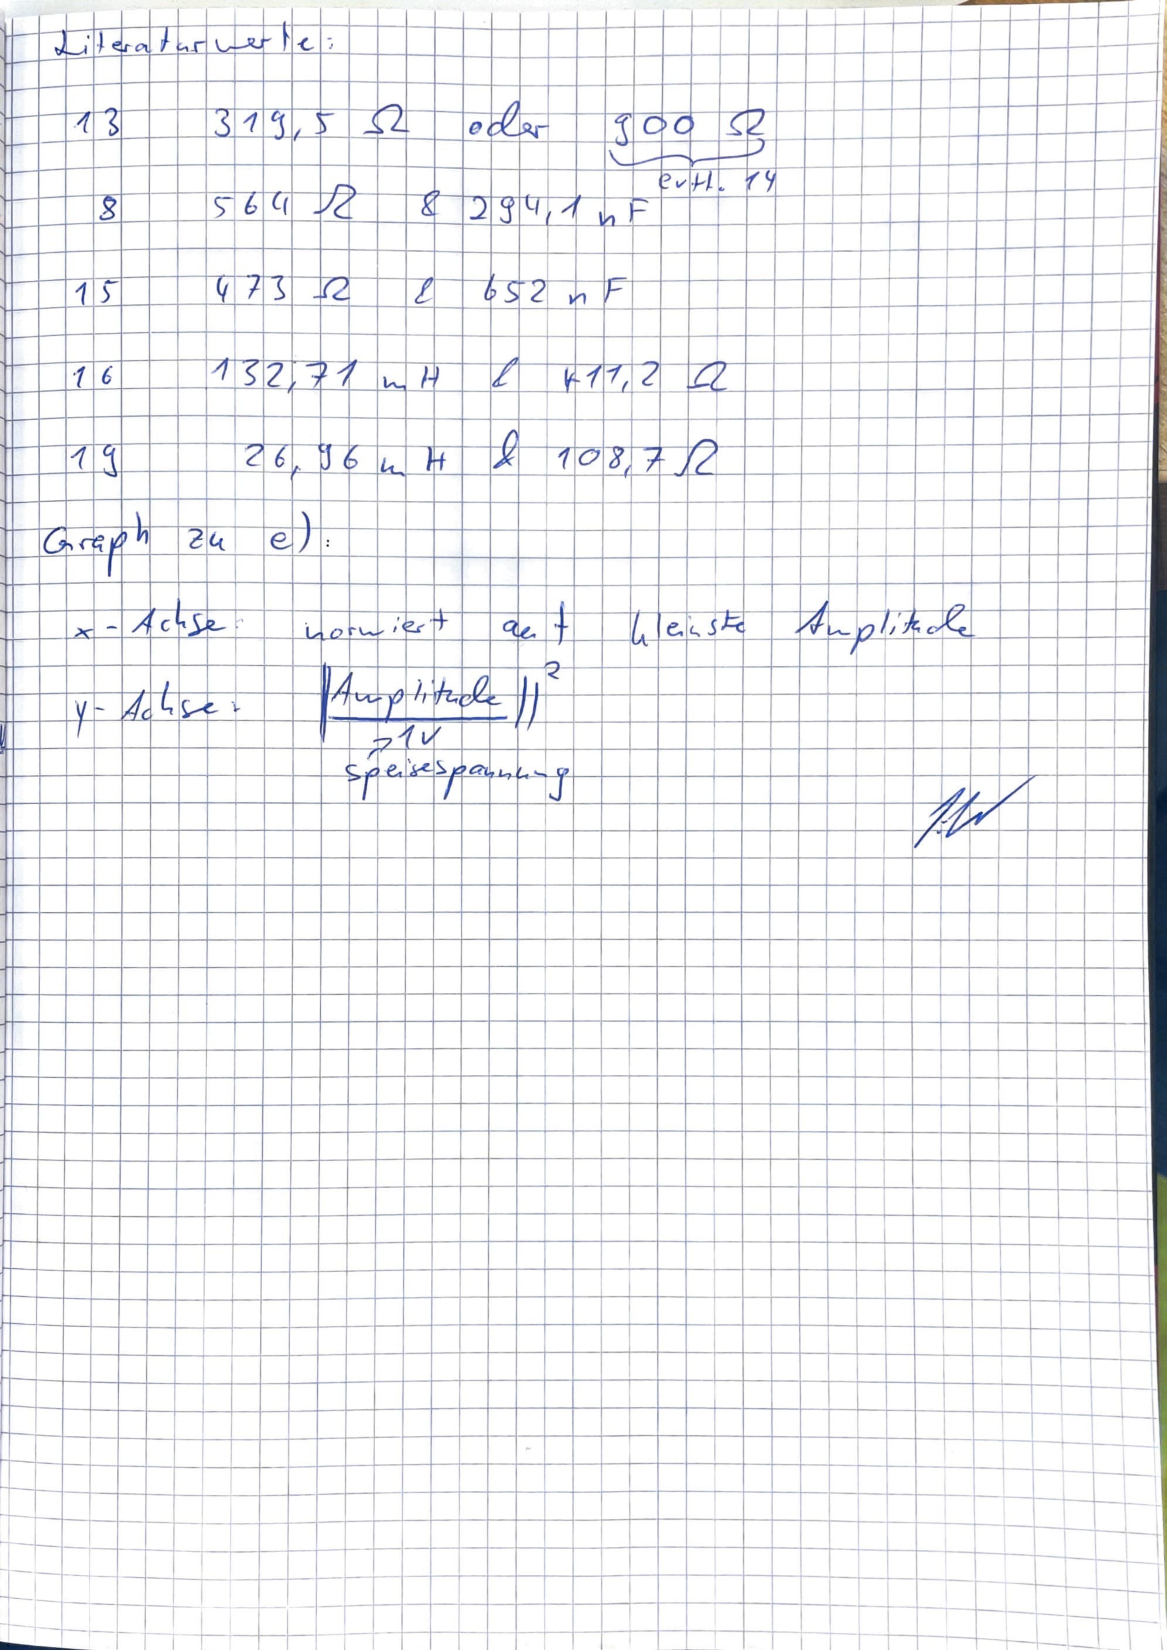
\includegraphics[width=\textwidth]{Messwerte_3.pdf}
    %   \label{fig:Messungen}
%\end{figure}

\printbibliography{}
\appendix
\setcounter{secnumdepth}{0}
\section{Anhang}
\label{sec:Anhang}
\subsection{Originaldaten}
%
\begin{figure}[H]
  \centering
  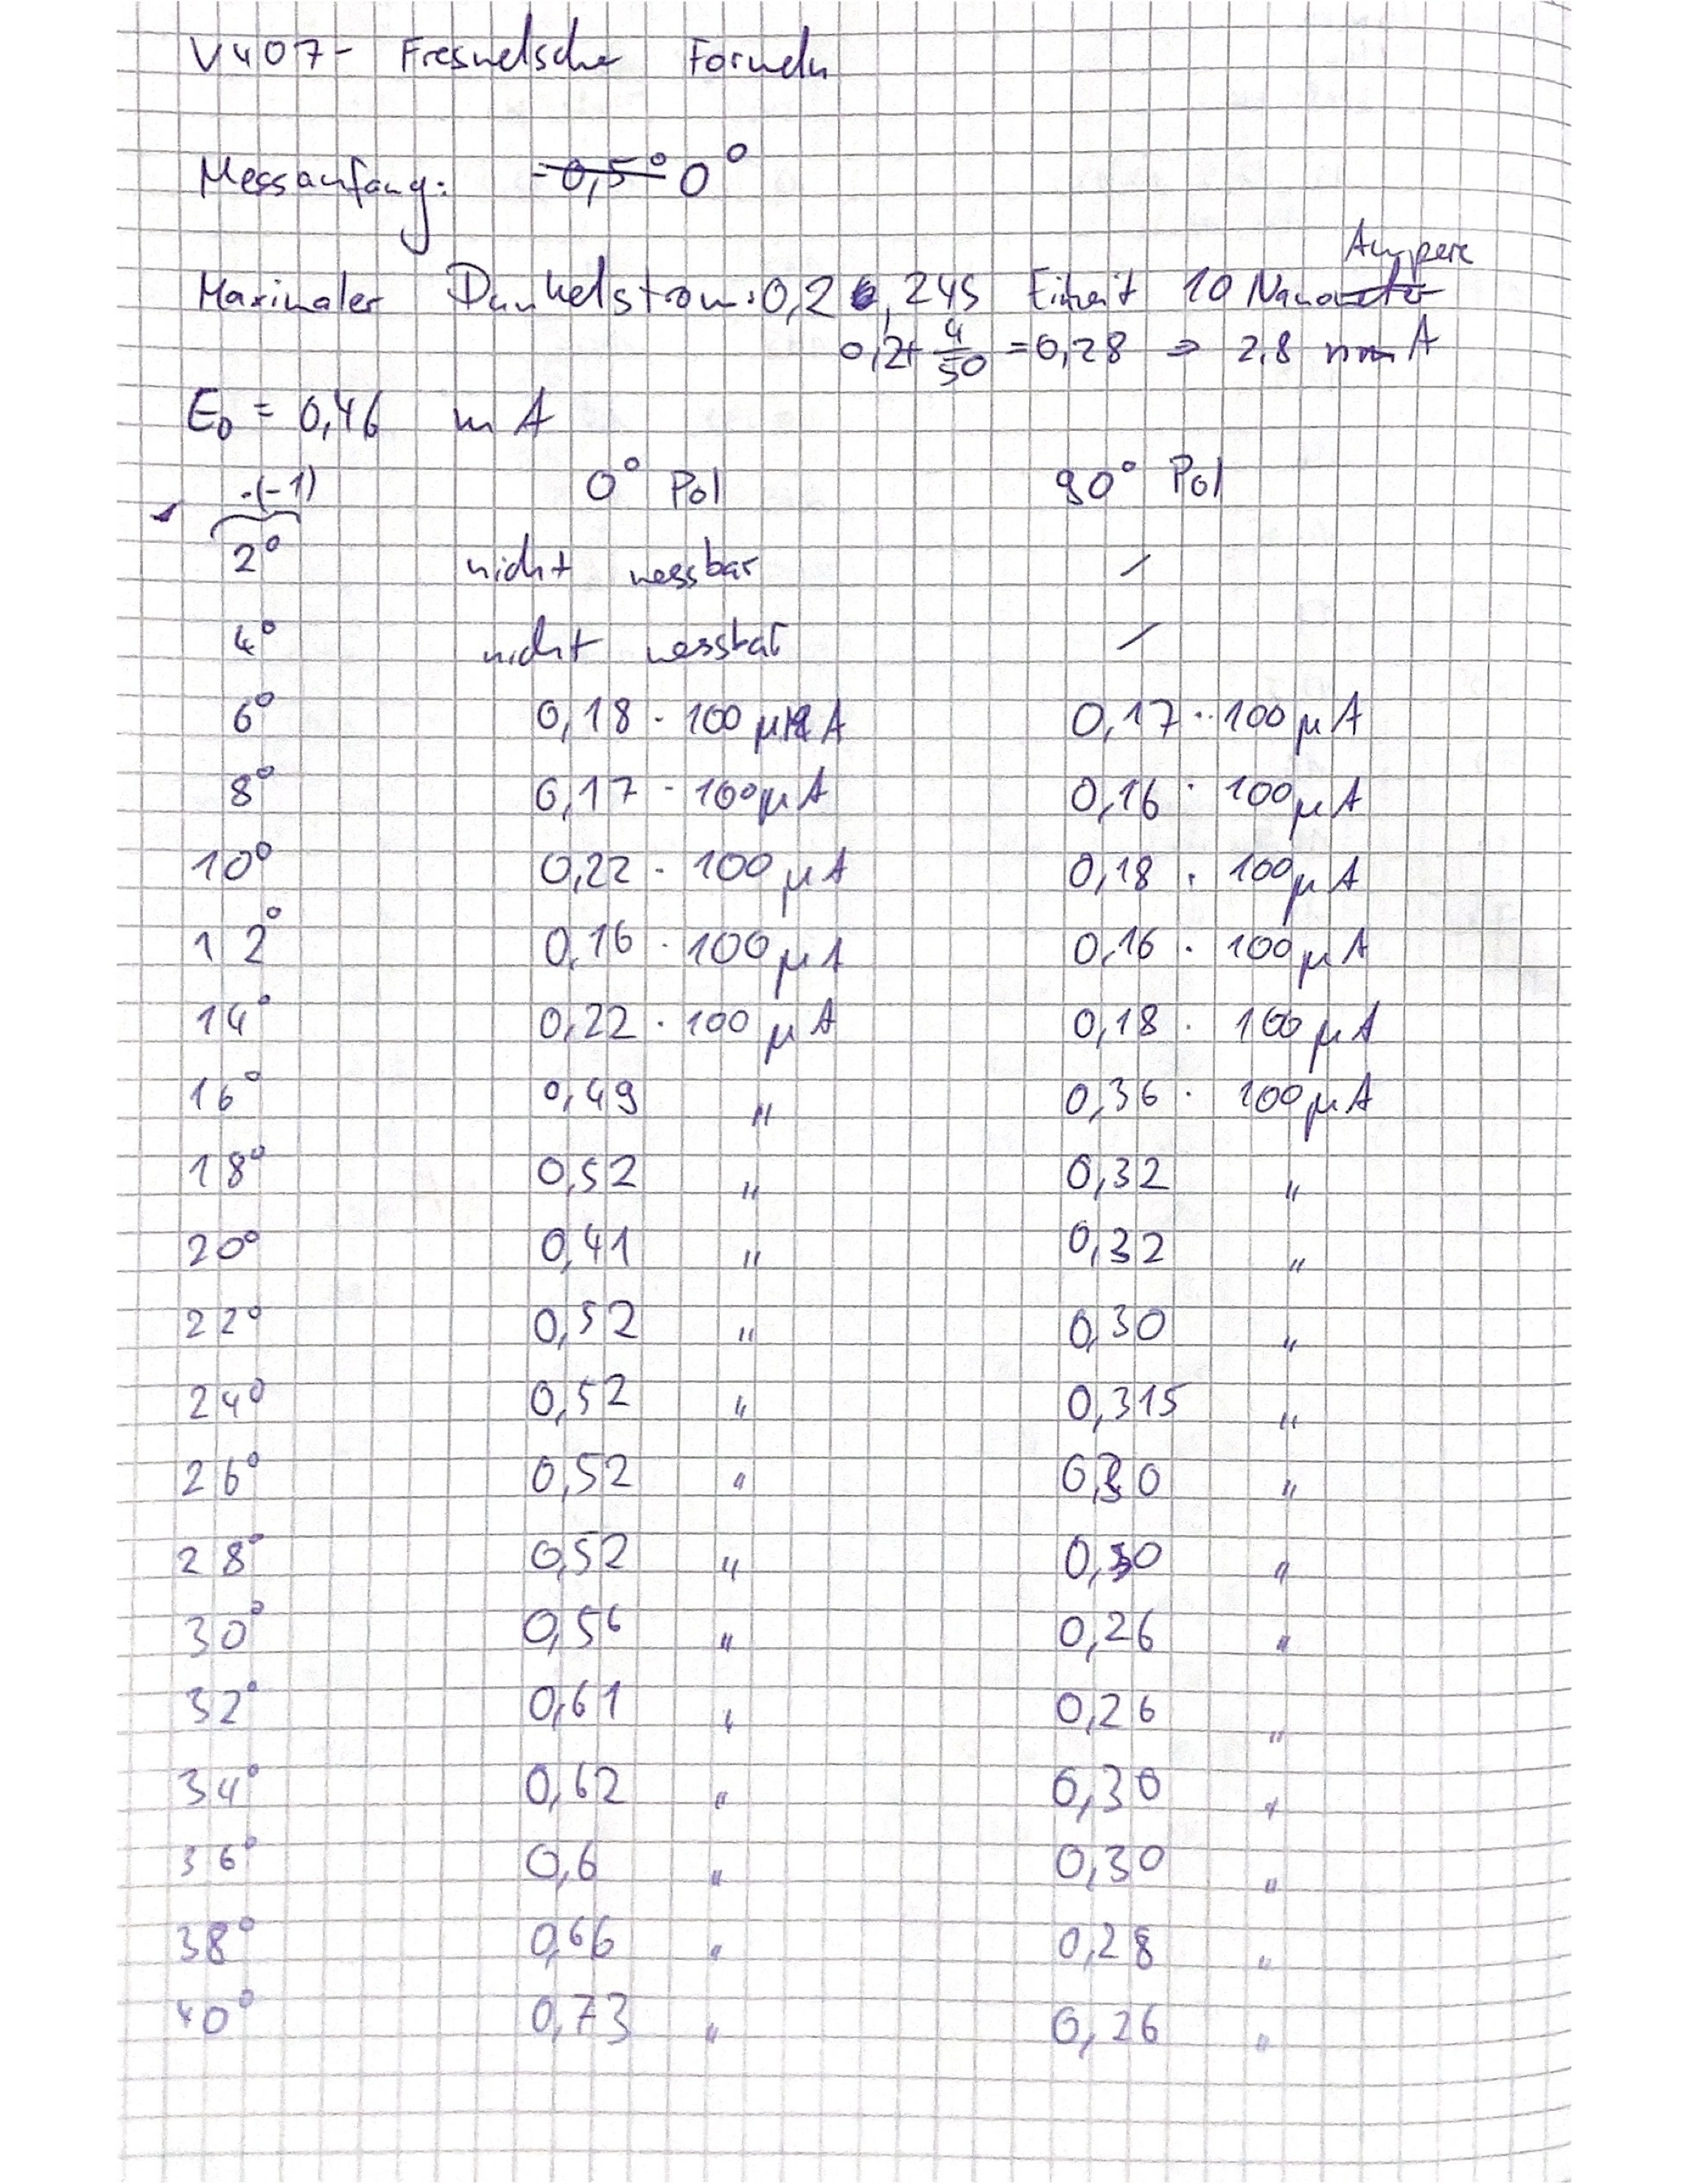
\includegraphics[width=0.8\textwidth]{content/Bilder/1.Blatt.jpeg}
  \label{fig:Messungen_1}
\end{figure}
\begin{figure}[H]
  \centering
  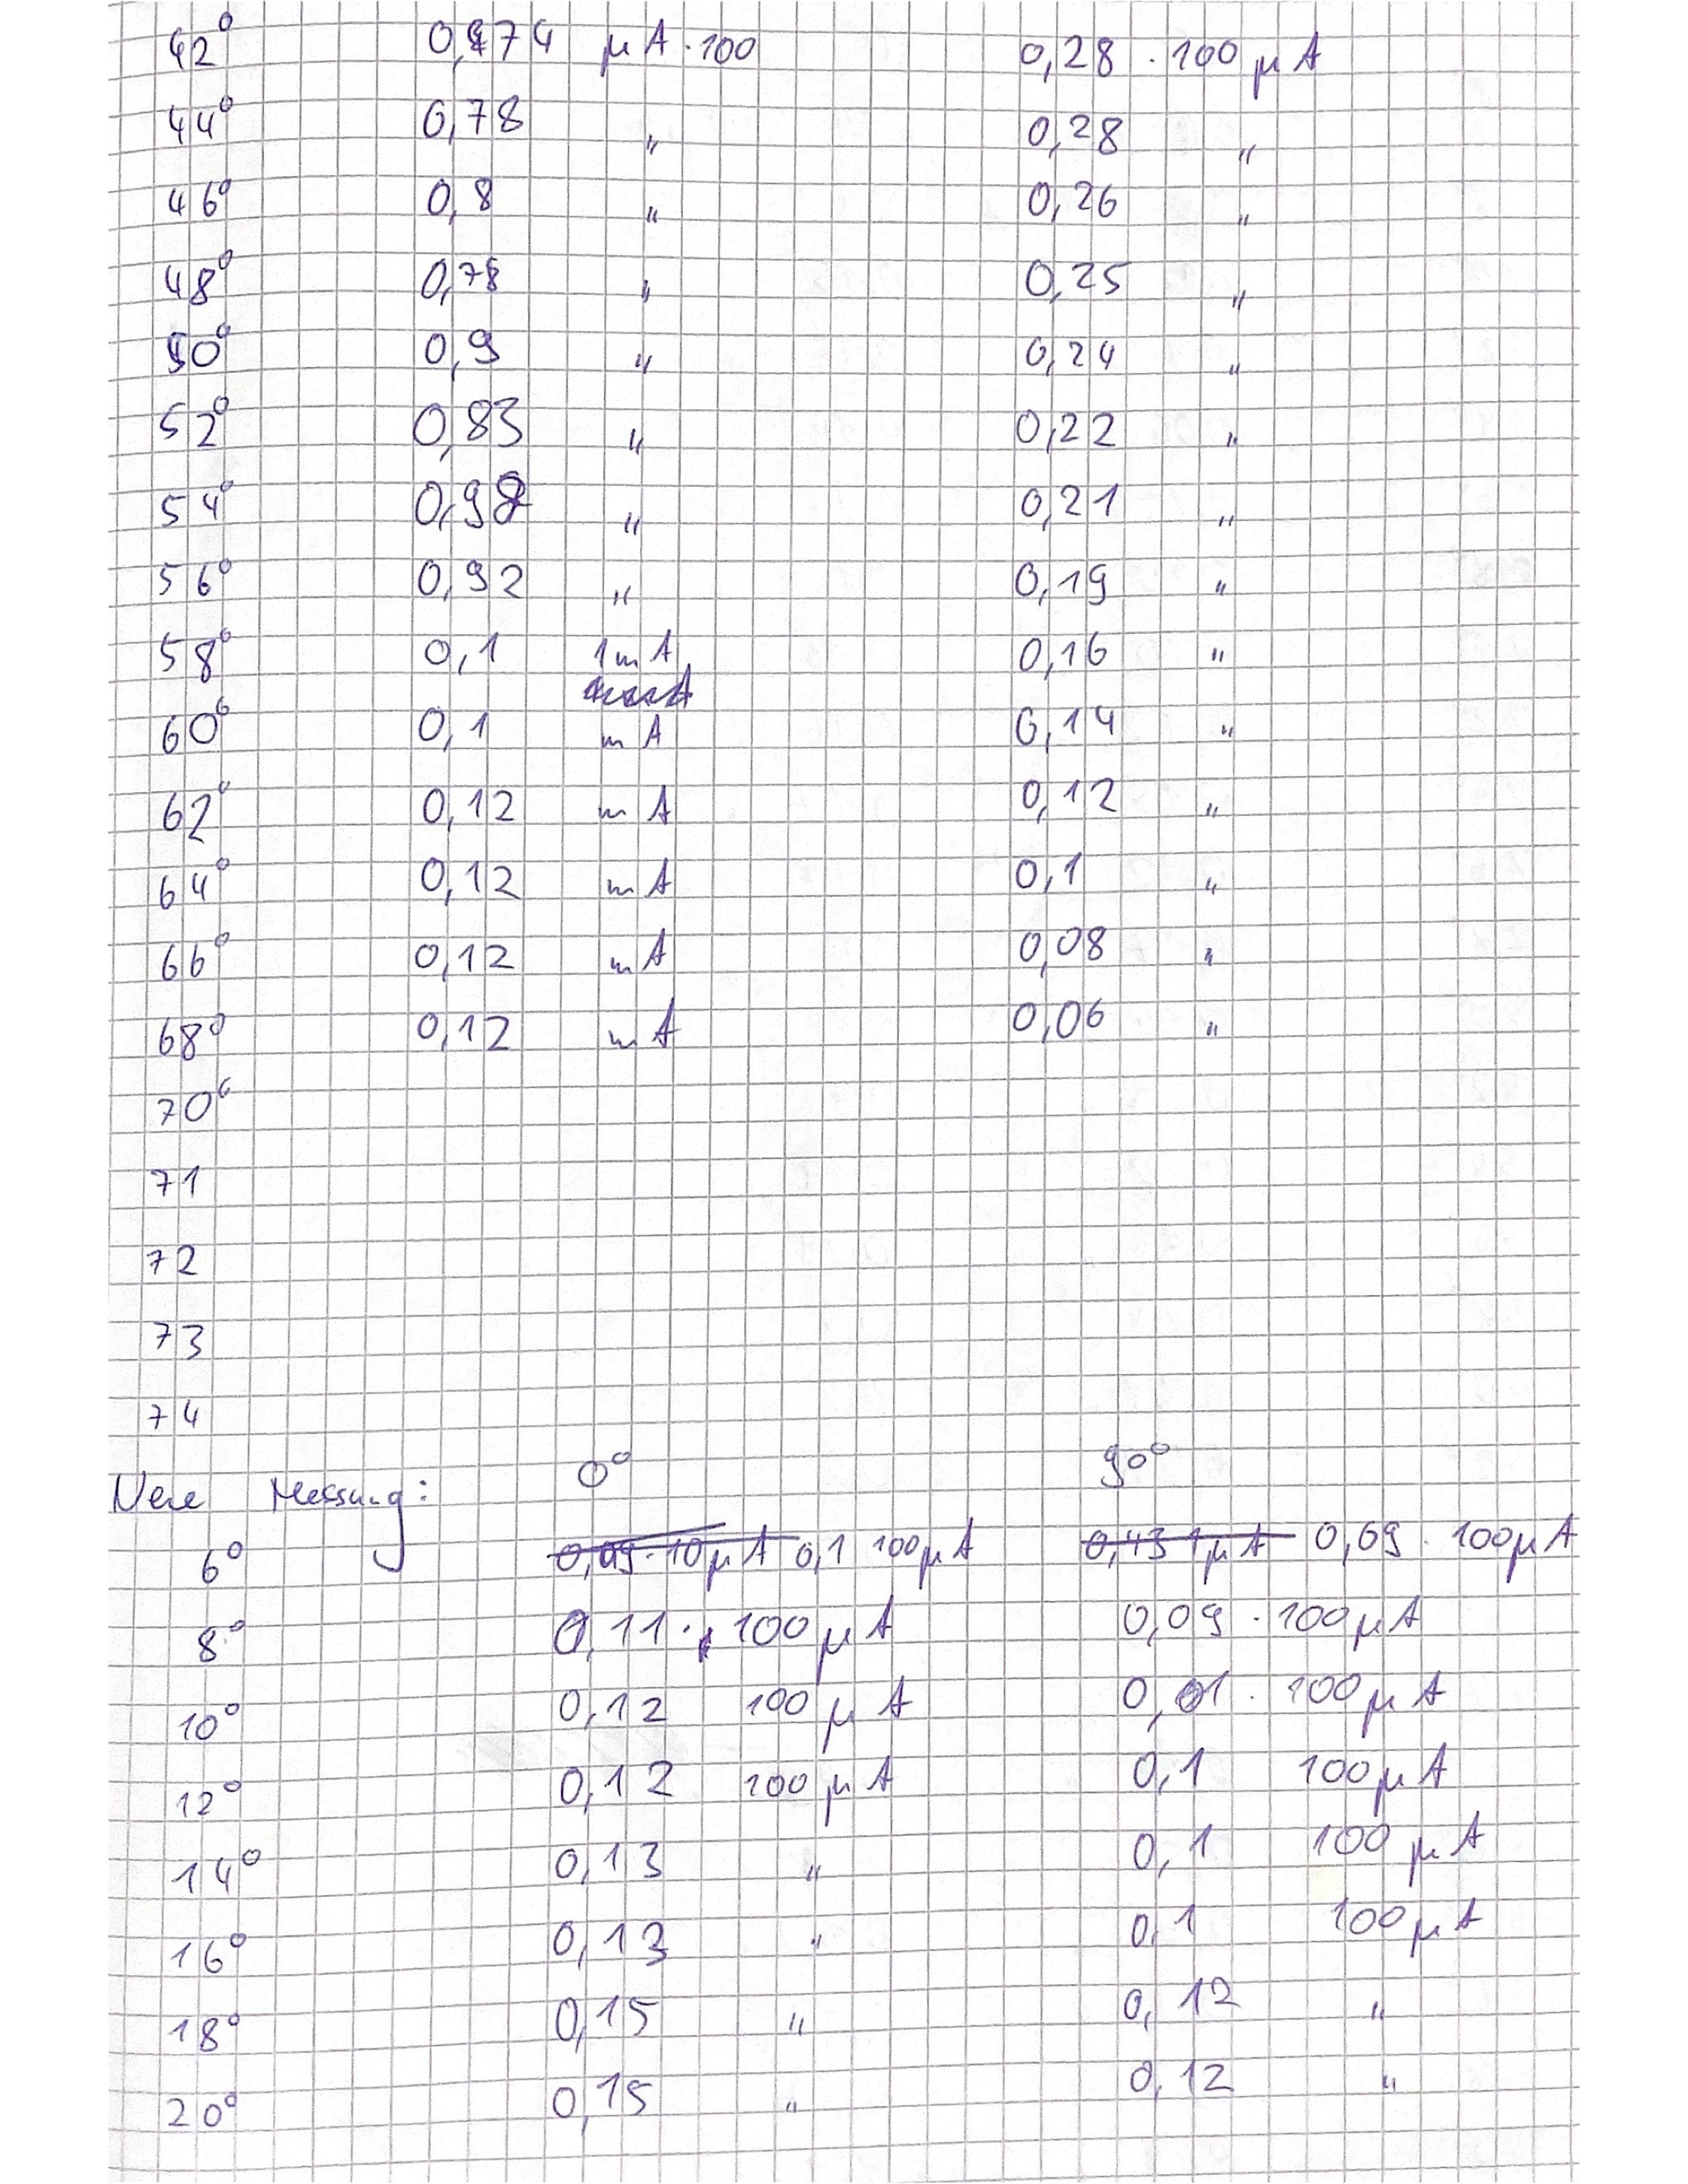
\includegraphics[width=\textwidth]{content/Bilder/2.Blatt.jpeg}
  \label{fig:Messungen_2}
\end{figure}
\begin{figure}[H]
  \centering
  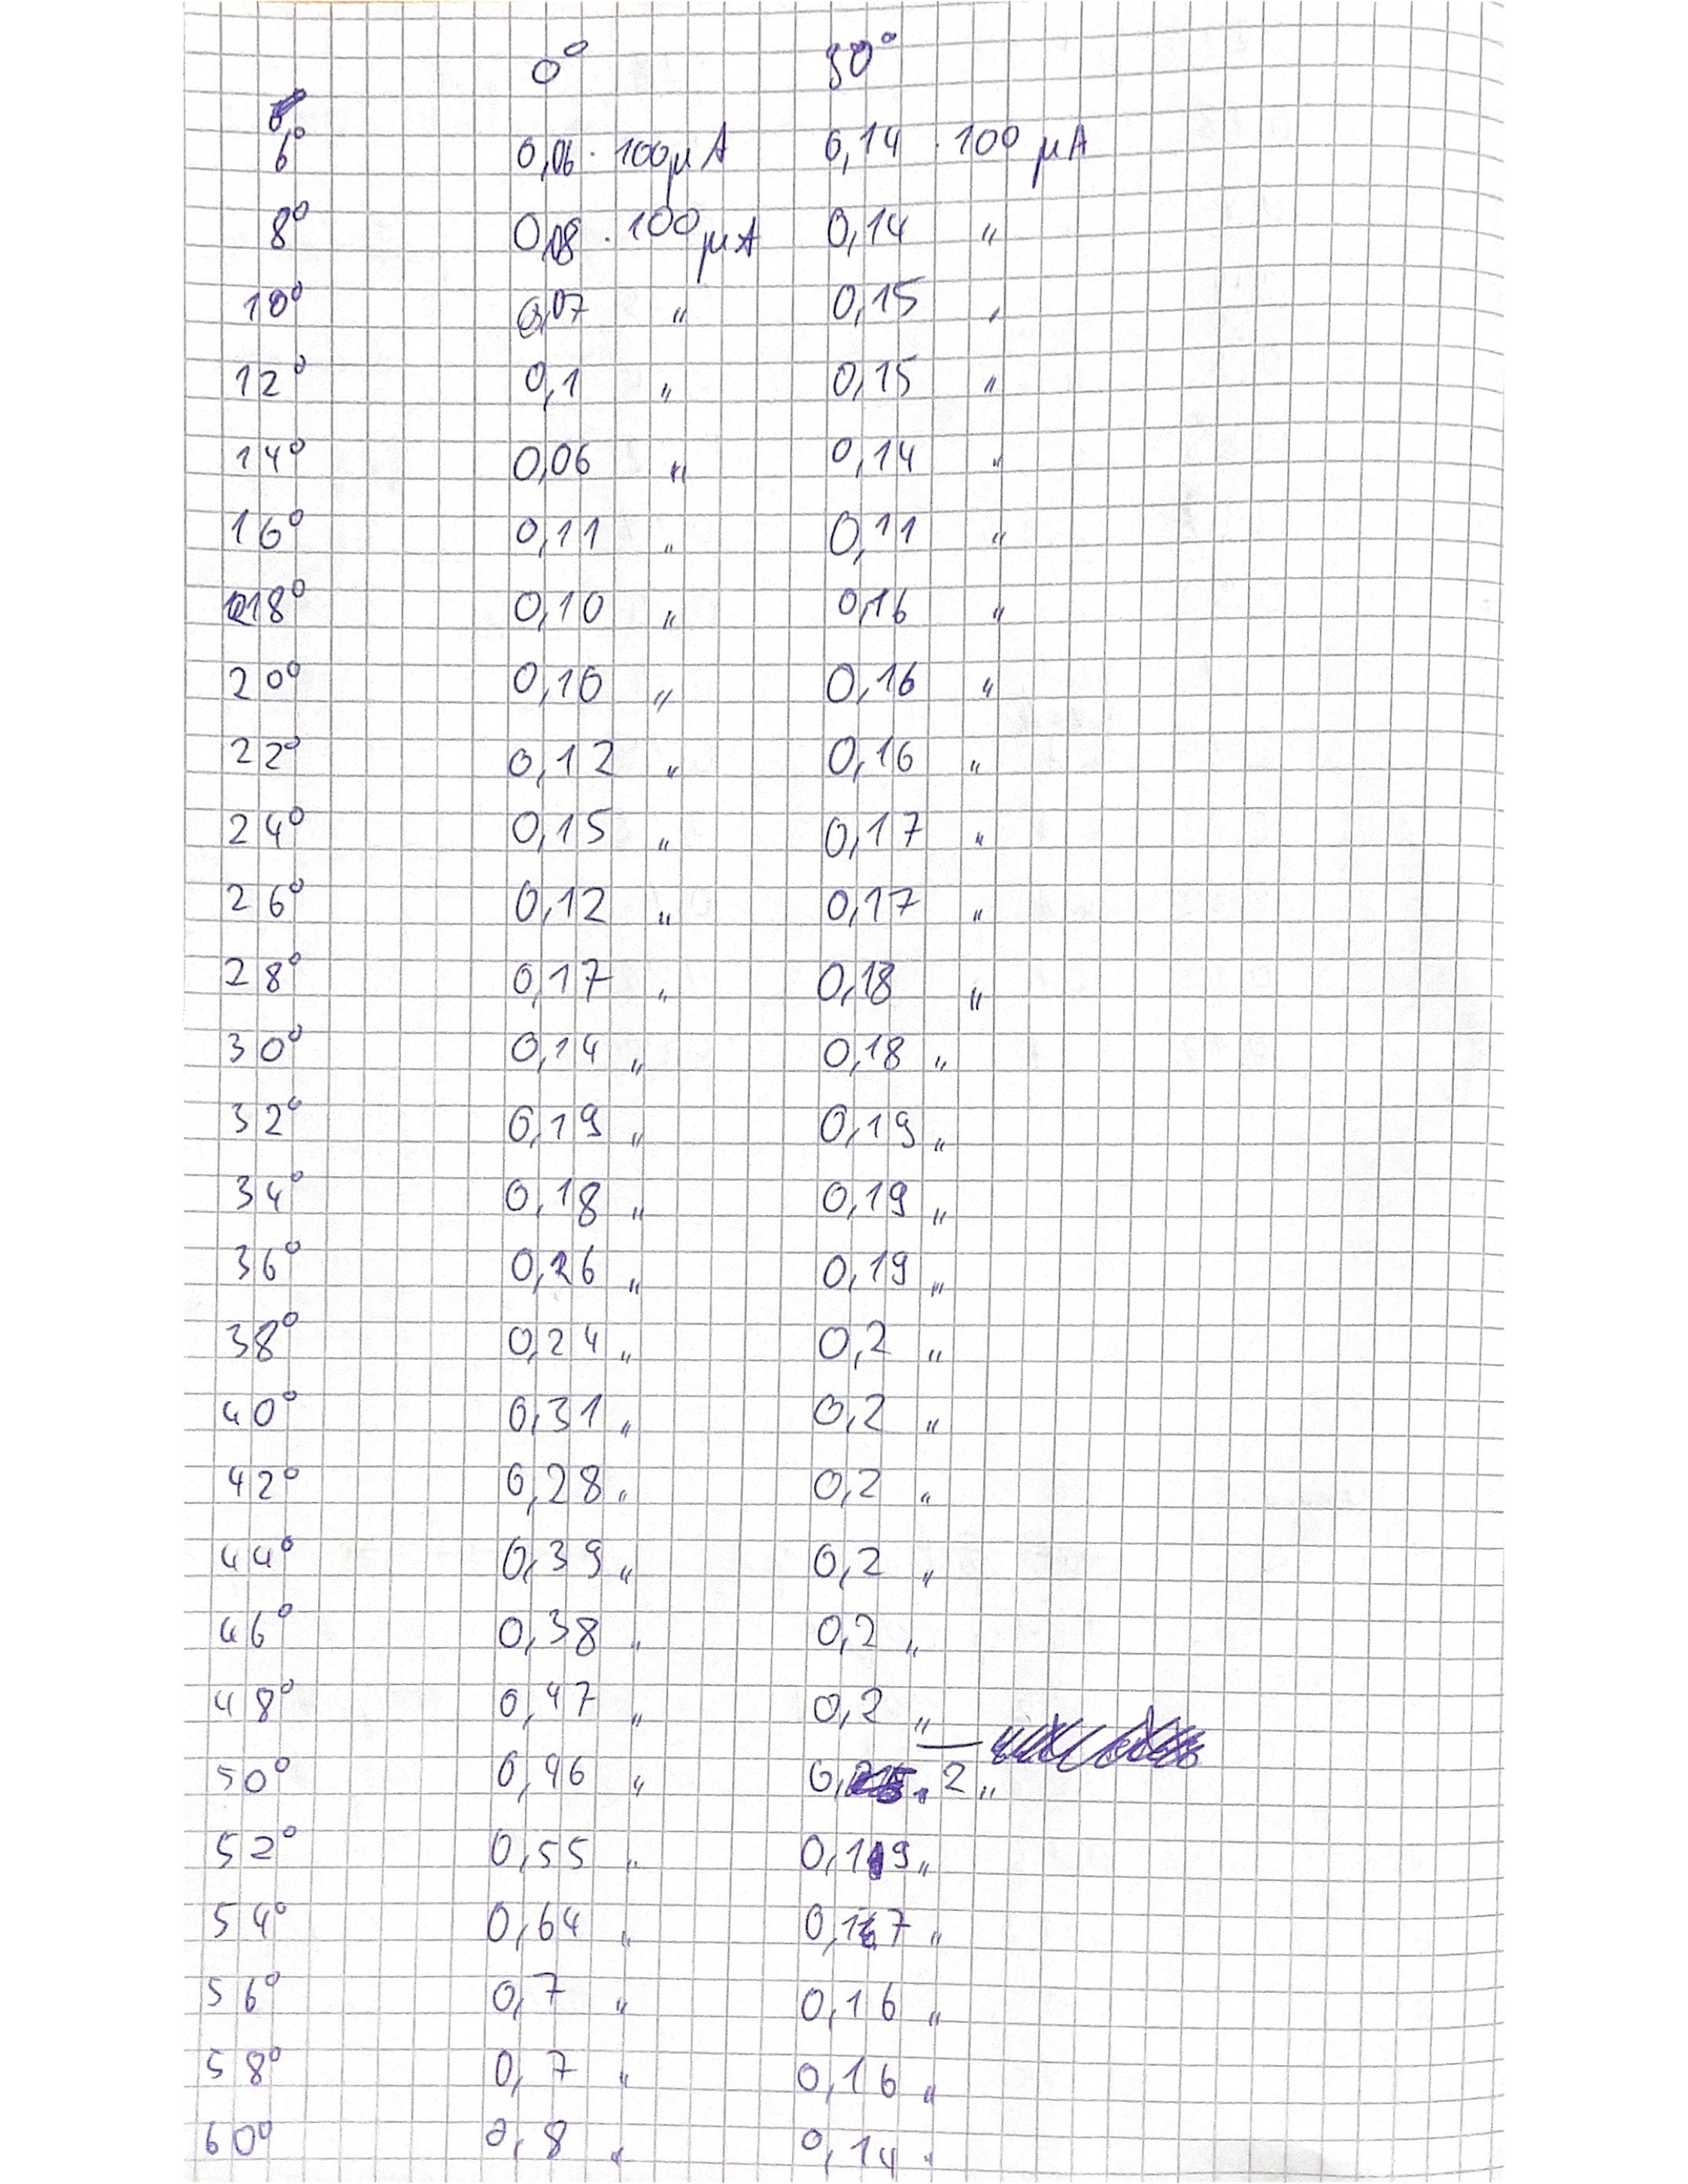
\includegraphics[width=\textwidth]{content/Bilder/3.Blatt.jpeg}
  \label{fig:Messungen_3}
\end{figure}
\begin{figure}[H]
    \centering
    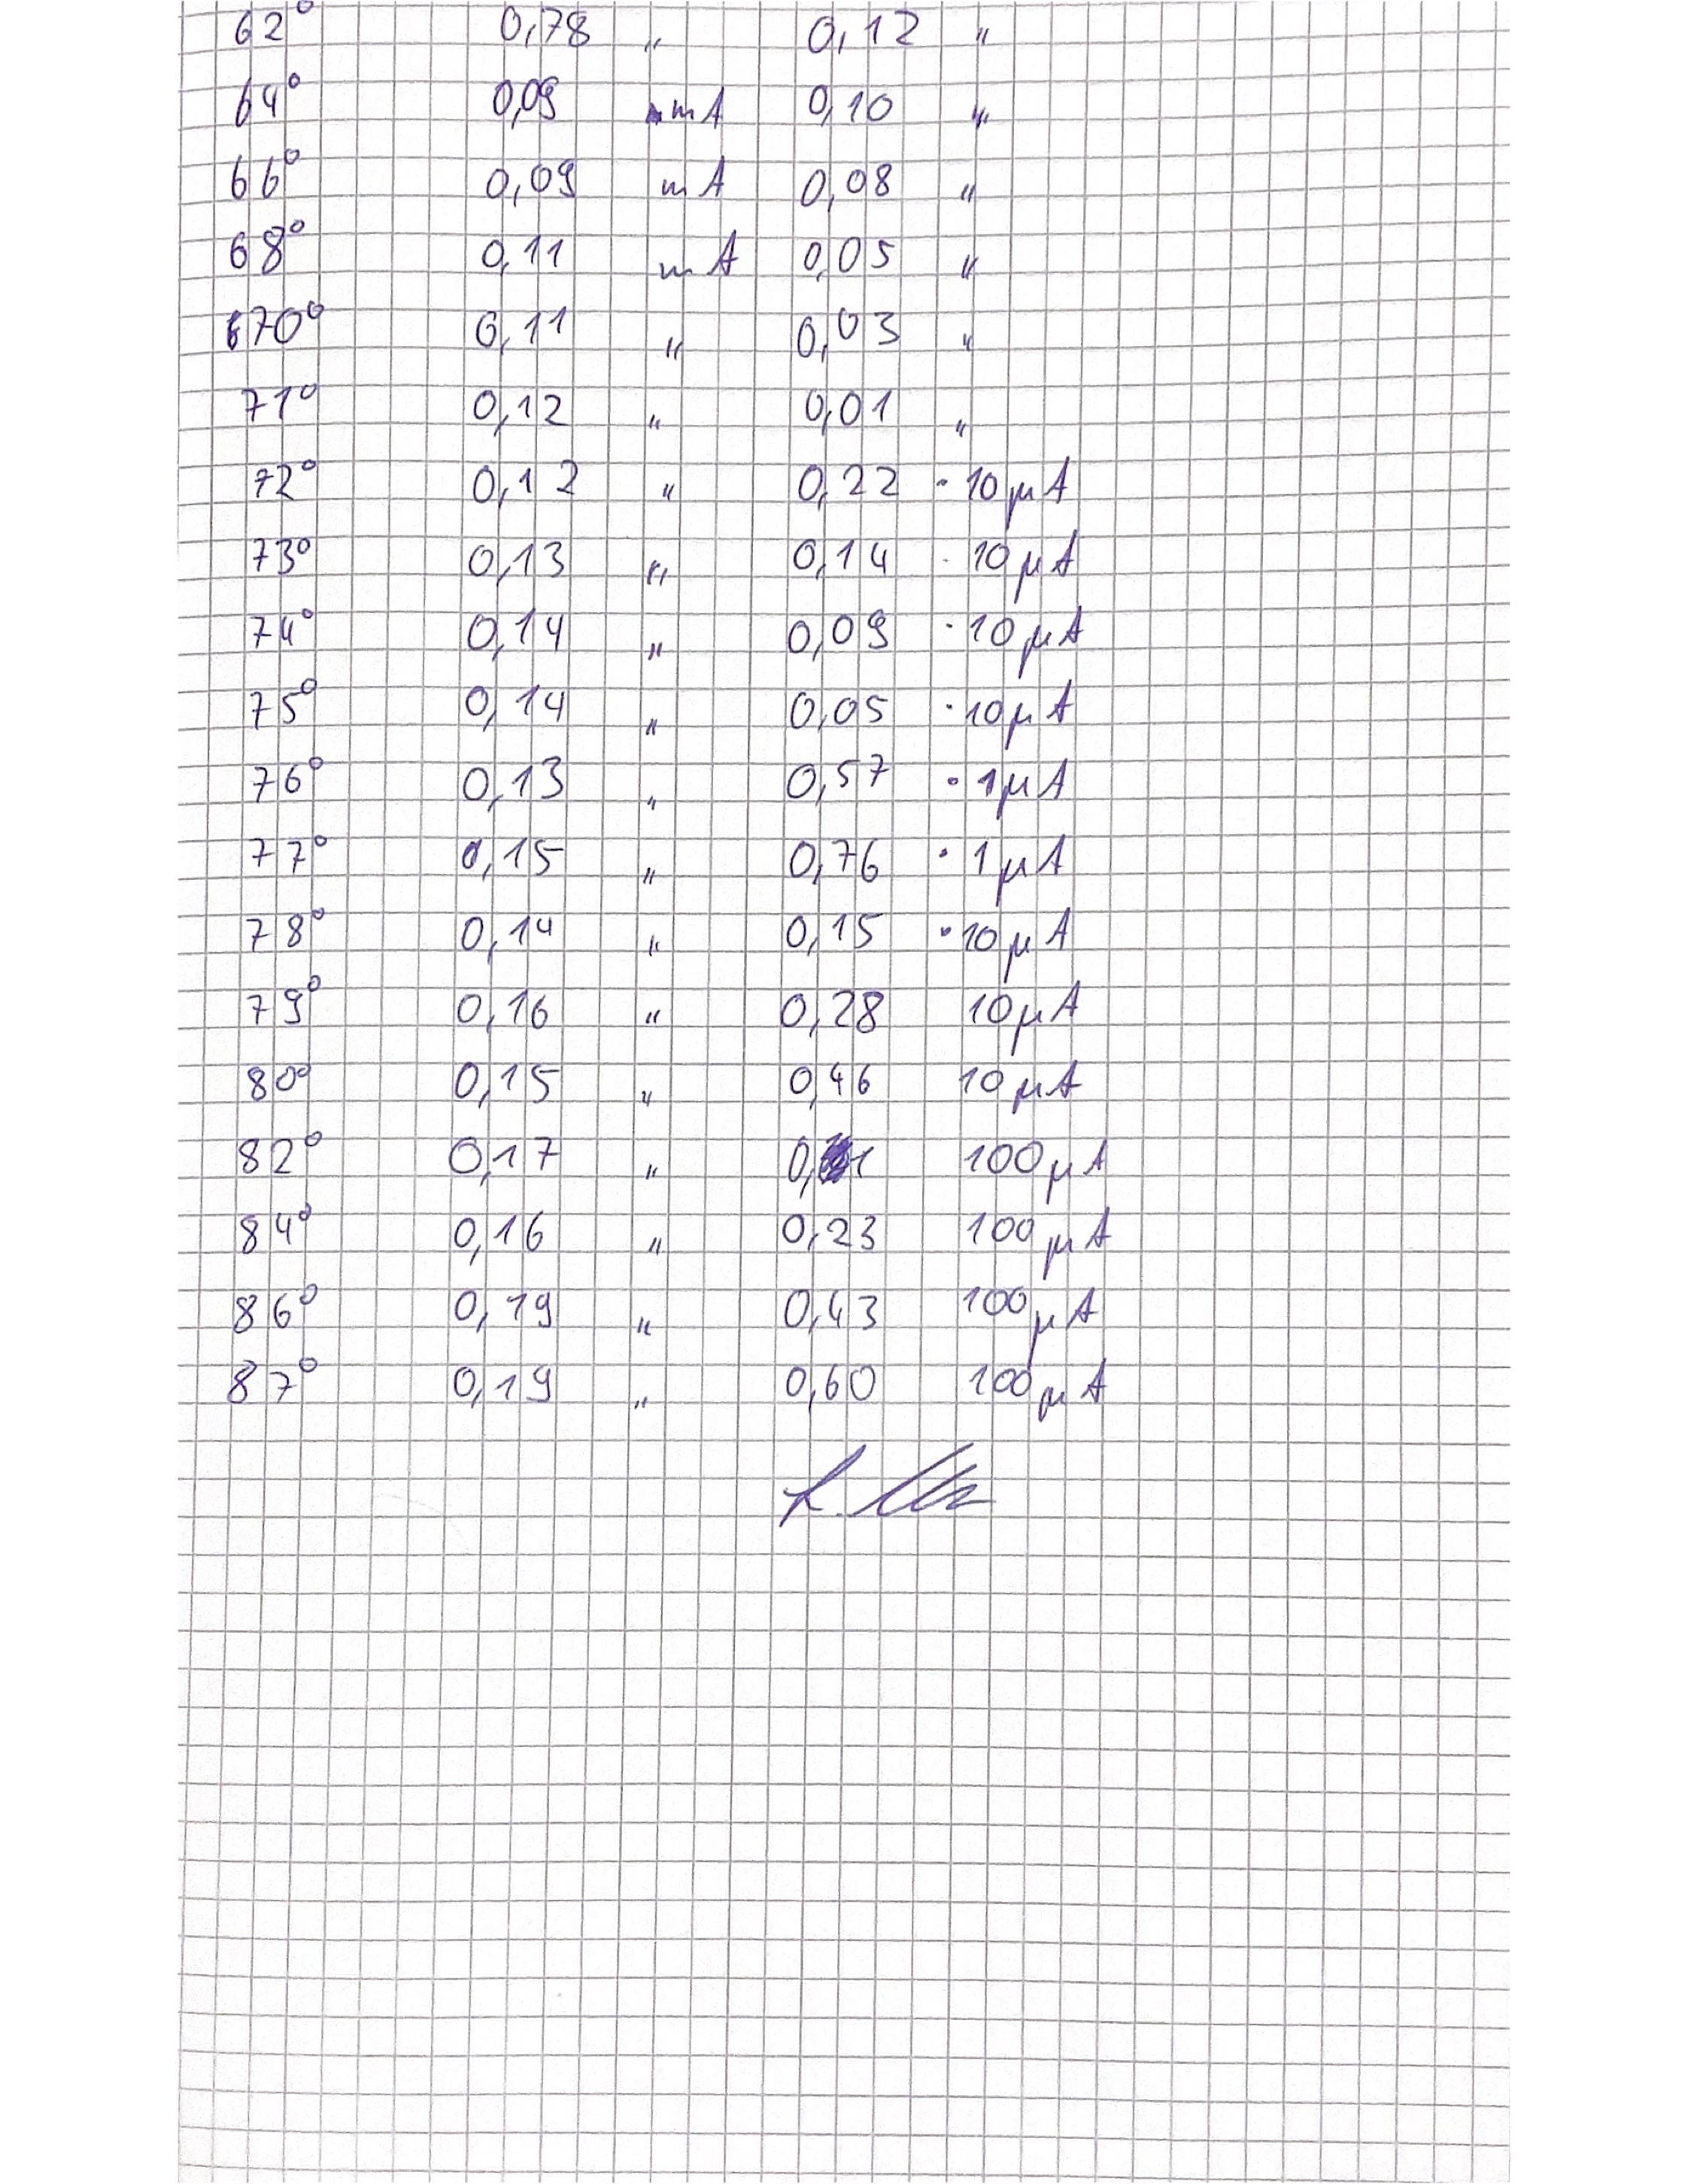
\includegraphics[width=\textwidth]{content/Bilder/4.Blatt.jpeg}
    \label{fig:Messungen_4}
  \end{figure}
\end{document}